\chapter{Исследовательская часть}

Цель исследования — разработка и реализация методов отбора значимых признаков для анализа и оценки близости документов, 
позволяющих уменьшить избыточность данных и повысить точность результатов.

\section{Оборудование}

Характеритстики ноутбука:
\begin{itemize}
	\item процессор intel-core i5-12500H \cite{lib:intel}
	\item ОЗУ 16 Гб DDR4
	\item ОС Windows 11 \cite{lib:windows}
\end{itemize}

\section{Результаты исследования}

Длина до всегда состаляет 6917 признаков, поэтому в таблице показывается только длина после.
\begin{table}[H]
    \centering
    \begin{tabular}{|l|c|c|}
    \hline
    \textbf{Метрика}                                  & \textbf{Длина после}             \\ \hline
    Дисперсия                                         & 558                              \\ \hline
    Математическое ожидание                           & 1322                             \\ \hline
    Ковариация                                        & 6805                             \\ \hline
    Пирсон                                            & 1600                             \\ \hline
    Спирмен                                           & 1443                             \\ \hline
    \end{tabular}
    \caption{Результаты сокращения векторов документов}
    \label{tab:similarity}
\end{table}

\begin{table}[H]
    \centering
    \begin{tabular}{|l|c|c|}
    \hline
    \textbf{Метрика}                                  & \textbf{Длина после}             \\ \hline
    Дисперсия                                         & 6917                             \\ \hline
    Математическое ожидание                           & 1233                             \\ \hline
    Ковариация                                        & 6849                             \\ \hline
    Пирсон                                            & 5824                             \\ \hline
    Спирмен                                           & 5816                             \\ \hline
    \end{tabular}
    \caption{Результаты сокращения векторов документов по тематике Анамнез}
    \label{tab:similarity}
\end{table}

\begin{table}[H]
    \centering
    \begin{tabular}{|l|c|c|}
    \hline
    \textbf{Метрика}                                  & \textbf{Длина после}             \\ \hline
    Дисперсия                                         & 5964                             \\ \hline
    Математическое ожидание                           & 1408                             \\ \hline
    Ковариация                                        & 6736                             \\ \hline
    Пирсон                                            & 5702                             \\ \hline
    Спирмен                                           & 5693                             \\ \hline
    \end{tabular}
    \caption{Результаты сокращения векторов документов по тематике Биохимия крови}
    \label{tab:similarity}
\end{table}

\begin{table}[H]
    \centering
    \begin{tabular}{|l|c|c|}
    \hline
    \textbf{Метрика}                                  & \textbf{Длина после}             \\ \hline
    Дисперсия                                         & 6917                             \\ \hline
    Математическое ожидание                           & 1054                             \\ \hline
    Ковариация                                        & 6823                             \\ \hline
    Пирсон                                            & 5974                             \\ \hline
    Спирмен                                           & 5972                             \\ \hline
    \end{tabular}
    \caption{Результаты сокращения векторов документов по тематике Комментаторы}
    \label{tab:similarity}
\end{table}

\begin{table}[H]
    \centering
    \begin{tabular}{|l|c|c|}
    \hline
    \textbf{Метрика}                                  & \textbf{Длина после}             \\ \hline
    Дисперсия                                         & 6917                             \\ \hline
    Математическое ожидание                           & 1439                             \\ \hline
    Ковариация                                        & 6757                             \\ \hline
    Пирсон                                            & 5621                             \\ \hline
    Спирмен                                           & 5613                             \\ \hline
    \end{tabular}
    \caption{Результаты сокращения векторов документов по тематике Неорганическая химия}
    \label{tab:similarity}
\end{table}

\begin{table}[H]
    \centering
    \begin{tabular}{|l|c|c|}
    \hline
    \textbf{Метрика}                                  & \textbf{Длина после}             \\ \hline
    Дисперсия                                         & 5820                             \\ \hline
    Математическое ожидание                           & 1445                             \\ \hline
    Ковариация                                        & 6796                             \\ \hline
    Пирсон                                            & 5592                             \\ \hline
    Спирмен                                           & 5579                             \\ \hline
    \end{tabular}
    \caption{Результаты сокращения векторов документов по тематике Органическая химия}
    \label{tab:similarity}
\end{table}

\begin{table}[H]
    \centering
    \begin{tabular}{|l|c|c|}
    \hline
    \textbf{Метрика}                                  & \textbf{Длина после}             \\ \hline
    Дисперсия                                         & 5719                             \\ \hline
    Математическое ожидание                           & 1454                             \\ \hline
    Ковариация                                        & 6804                             \\ \hline
    Пирсон                                            & 5894                             \\ \hline
    Спирмен                                           & 5881                             \\ \hline
    \end{tabular}
    \caption{Результаты сокращения векторов документов по тематике Спортивная медицина}
    \label{tab:similarity}
\end{table}

\begin{figure}[H]
    \begin{minipage}[H]{0.5\linewidth}
        \center{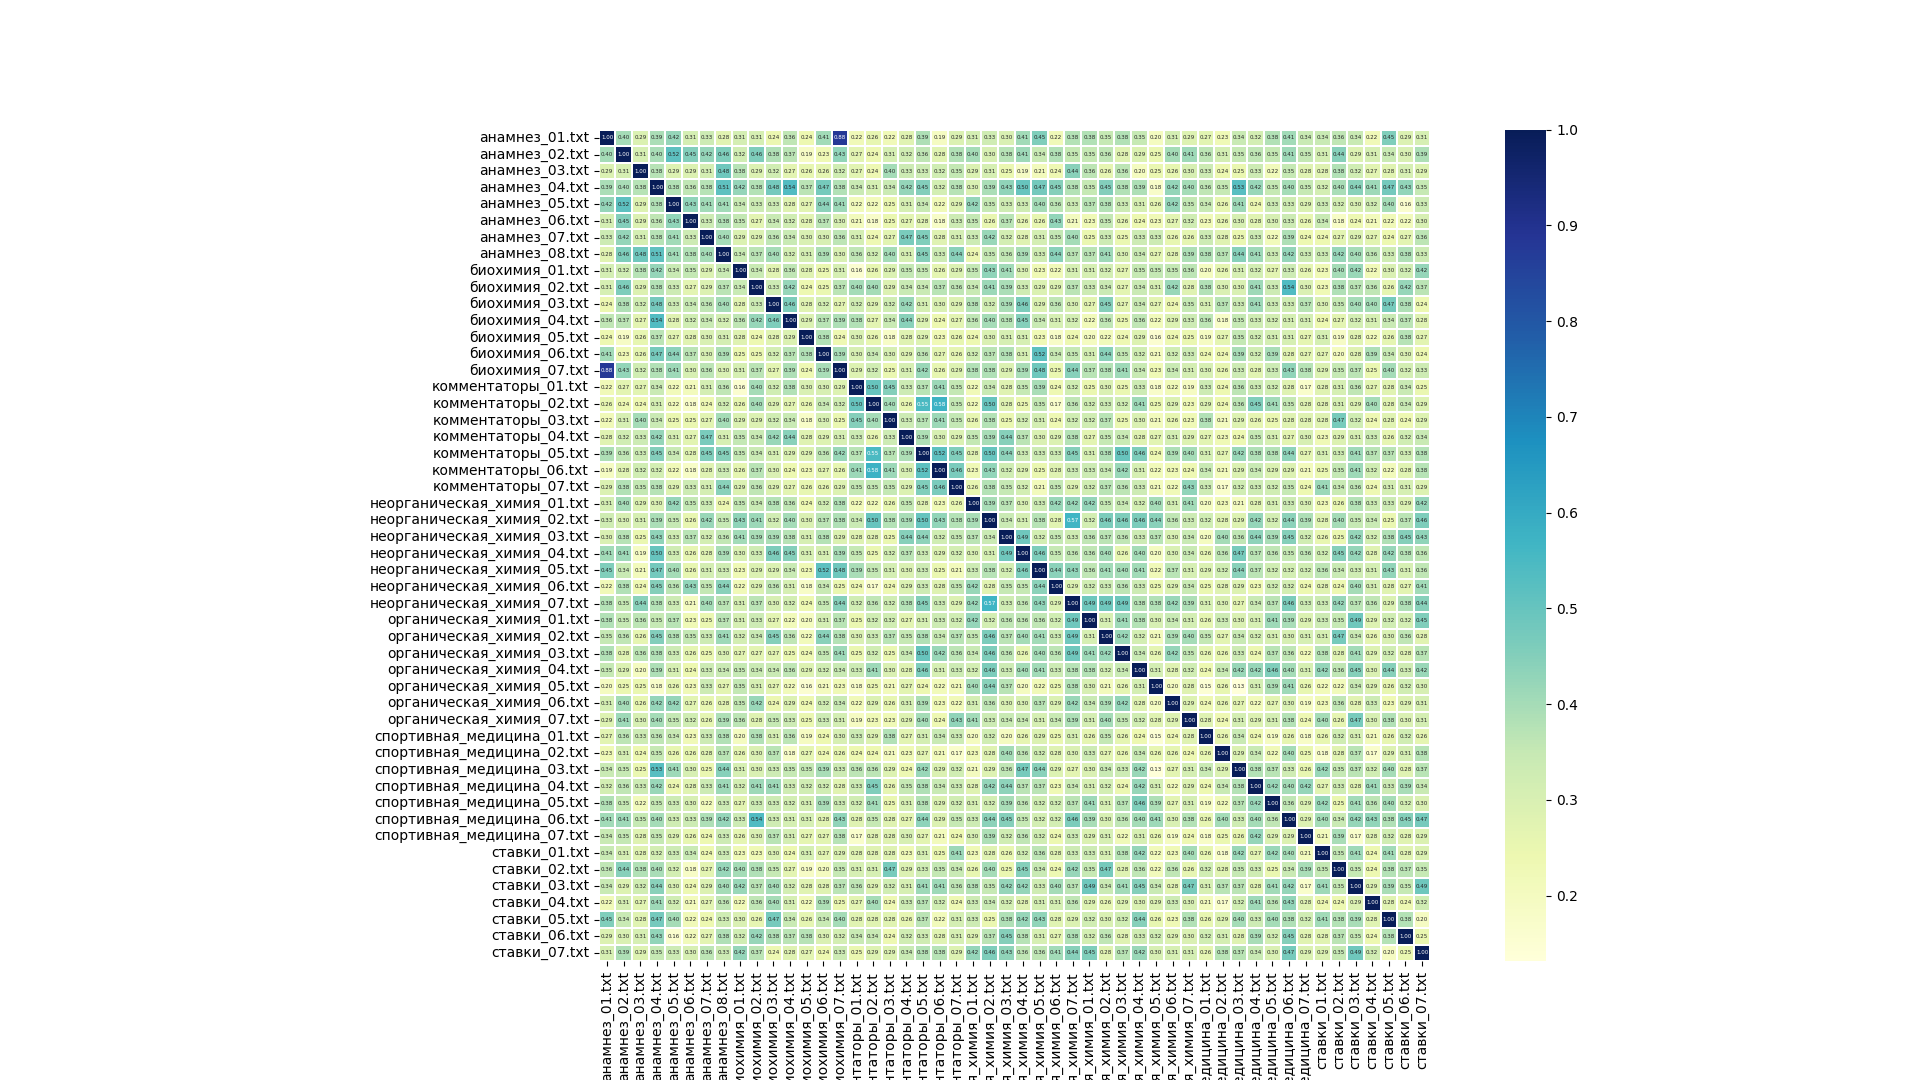
\includegraphics[width=1.1\linewidth]{C:/MGTU/baseAI/lr8_git/bag23u045/report/images/HeatmapJac.png}}
        а) До сокращения вектора 
    \end{minipage}
    \begin{minipage}[H]{0.5\linewidth}
        \center{\includegraphics[width=1.1\linewidth]{C:/MGTU/baseAI/lr10/bag23u045/report/results/Heatmap_mean_jac.png}}
        б) После сокращения вектора 
    \end{minipage}
    \caption{Сравнение методом Жаккарда уменьшенного вектора с помощью среднего значения}
    \label{fig:heatmapMeanJac}
\end{figure}

\begin{figure}[H]
    \begin{minipage}[H]{0.5\linewidth}
        \center{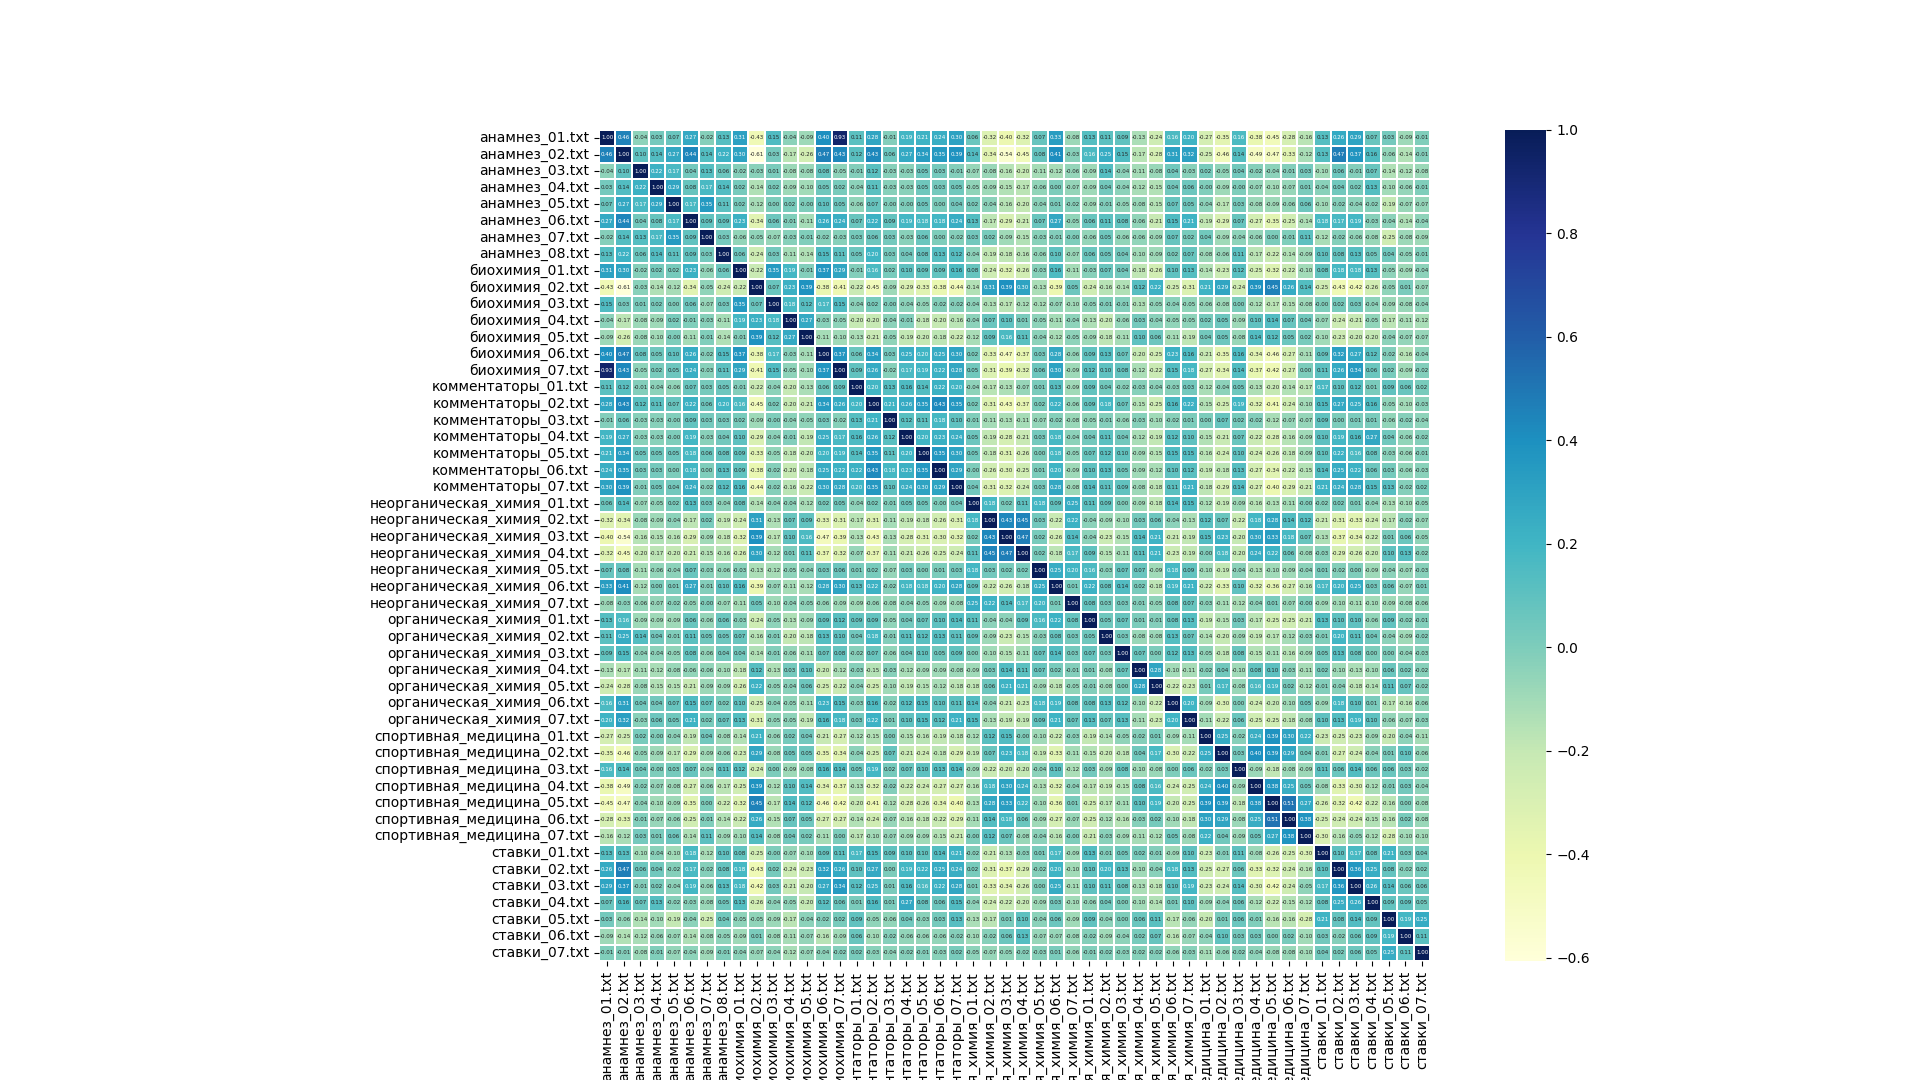
\includegraphics[width=1.1\linewidth]{C:/MGTU/baseAI/lr8_git/bag23u045/report/images/HeatmapCos.png}}
        а) До сокращения вектора 
    \end{minipage}
    \begin{minipage}[H]{0.5\linewidth}
        \center{\includegraphics[width=1.1\linewidth]{C:/MGTU/baseAI/lr10/bag23u045/report/results/Heatmap_mean_cosine.png}}
        б) После сокращения вектора 
    \end{minipage}
    \caption{Сравнение косинусным методом уменьшенного вектора с помощью среднего значения}
    \label{fig:heatmapMeanCosine}
\end{figure}

\begin{figure}[H]
    \begin{minipage}[H]{0.5\linewidth}
        \center{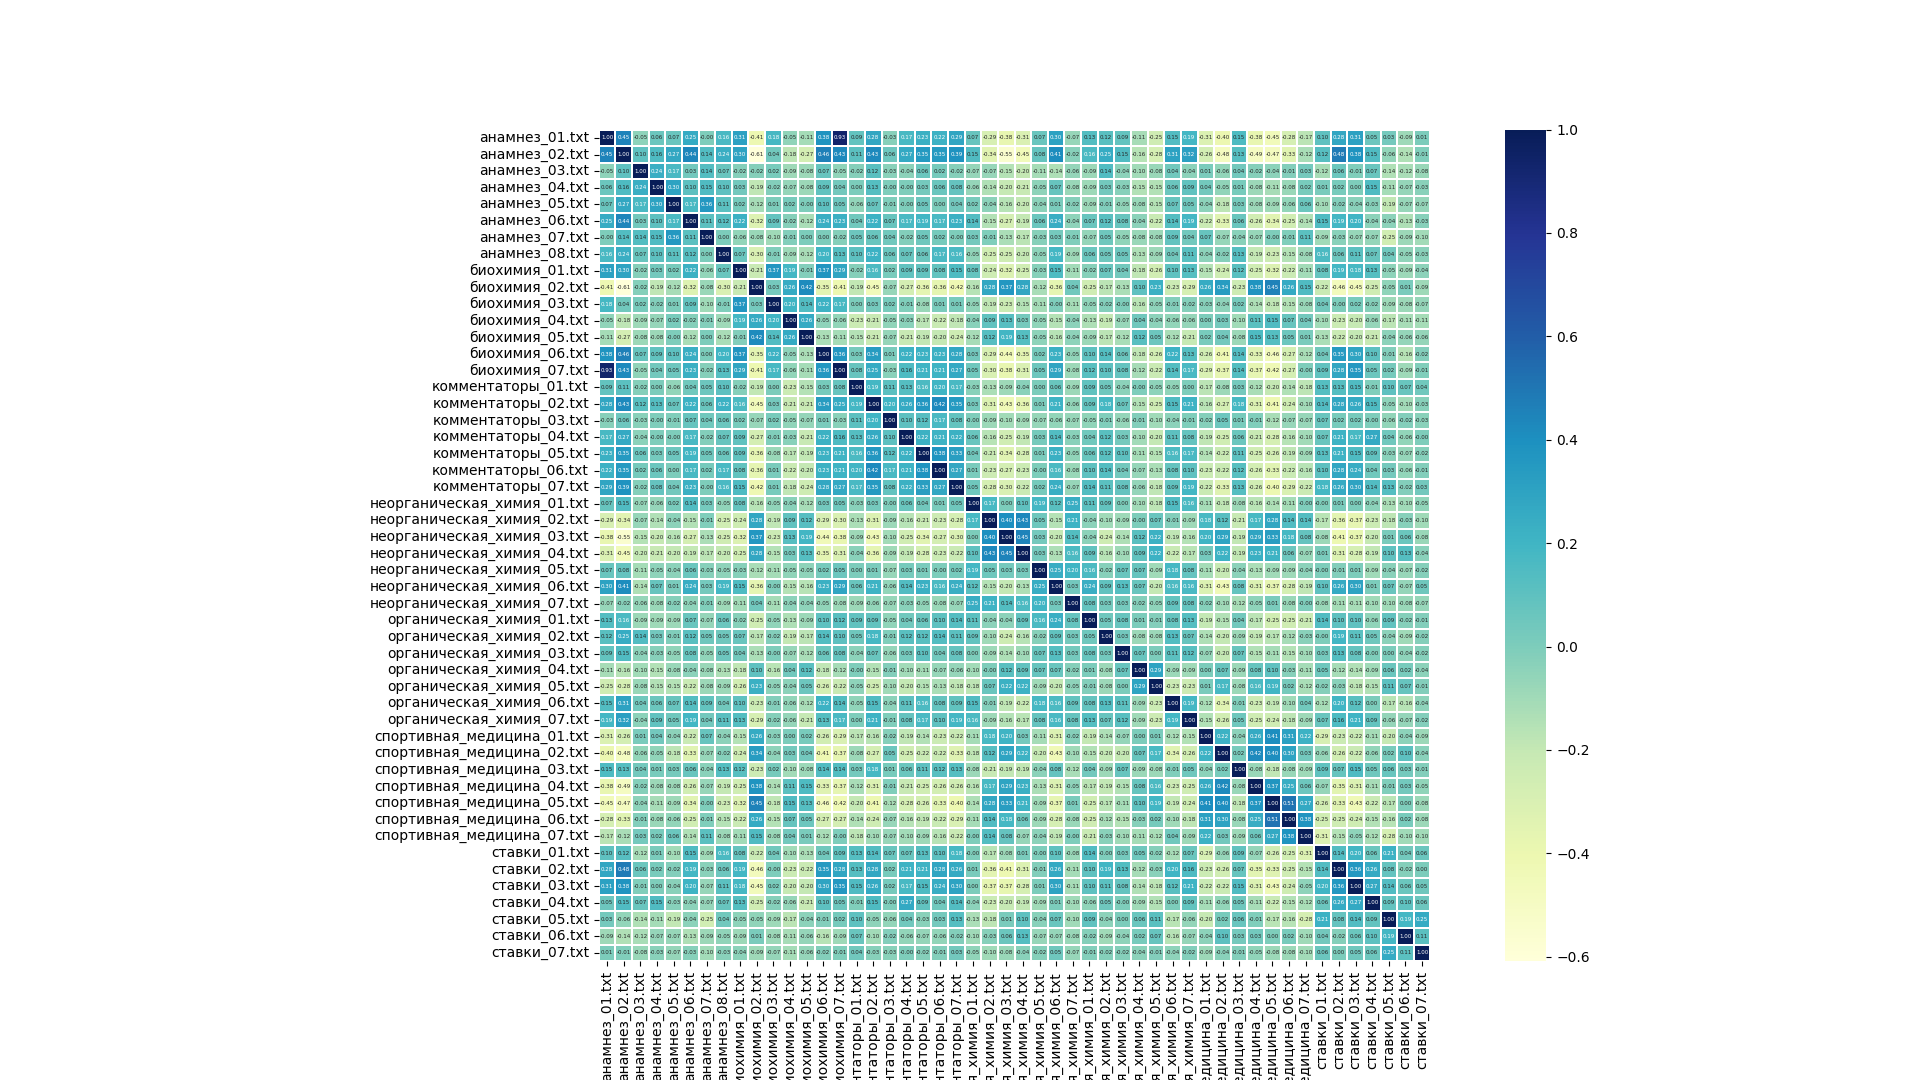
\includegraphics[width=1.1\linewidth]{C:/MGTU/baseAI/lr8_git/bag23u045/report/images/HeatmapPearson.png}}
        а) До сокращения вектора 
    \end{minipage}
    \begin{minipage}[H]{0.5\linewidth}
        \center{\includegraphics[width=1.1\linewidth]{C:/MGTU/baseAI/lr10/bag23u045/report/results/Heatmap_mean_pearson.png}}
        б) После сокращения вектора 
    \end{minipage}
    \caption{Сравнение методом Пирсона уменьшенного вектора с помощью среднего значения}
    \label{fig:heatmapMeanPearson}
\end{figure}

\begin{figure}[H]
    \begin{minipage}[H]{0.5\linewidth}
        \center{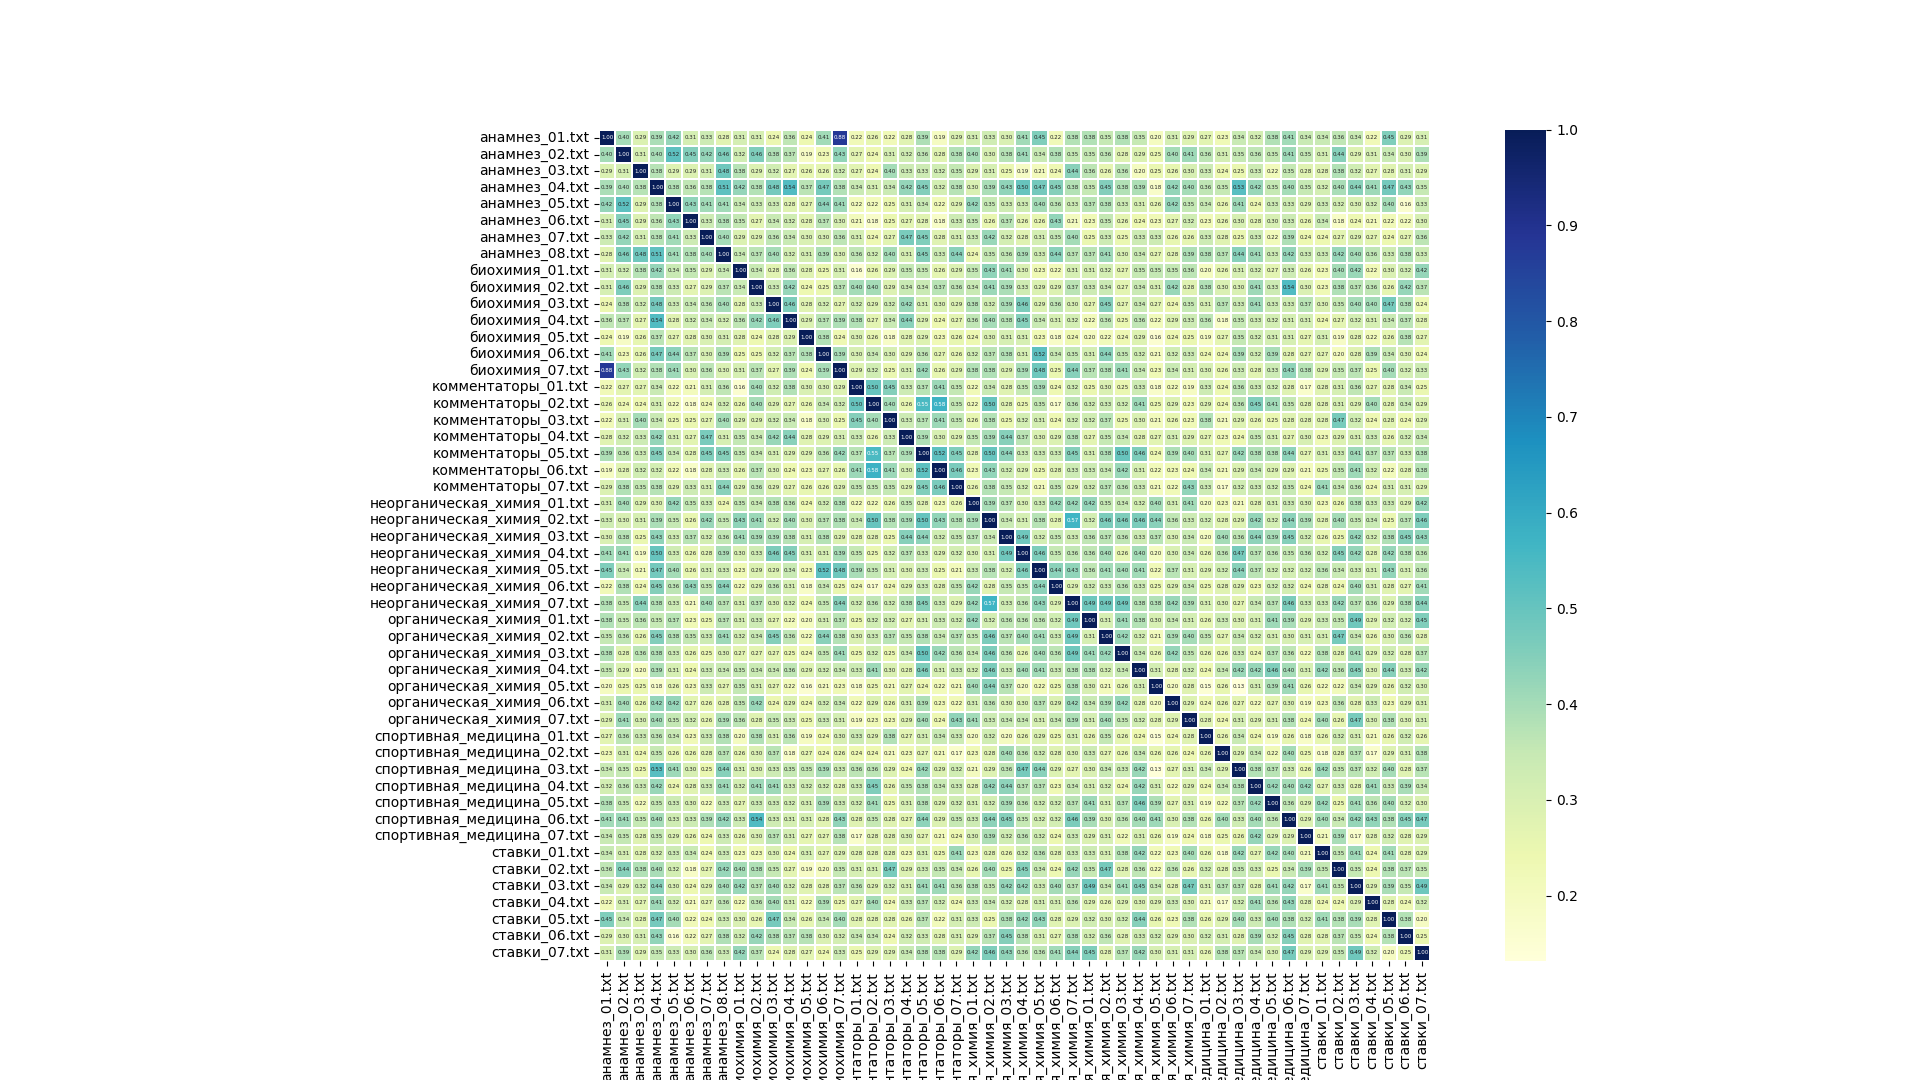
\includegraphics[width=1.1\linewidth]{C:/MGTU/baseAI/lr8_git/bag23u045/report/images/HeatmapJac.png}}
        а) До сокращения вектора 
    \end{minipage}
    \begin{minipage}[H]{0.5\linewidth}
        \center{\includegraphics[width=1.1\linewidth]{C:/MGTU/baseAI/lr10/bag23u045/report/results/Heatmap_dispersion_jac.png}}
        б) После сокращения вектора 
    \end{minipage}
    \caption{Сравнение методом Жаккарда уменьшенного вектора с помощью диспресии}
    \label{fig:heatmapVarJac}
\end{figure}

\begin{figure}[H]
    \begin{minipage}[H]{0.5\linewidth}
        \center{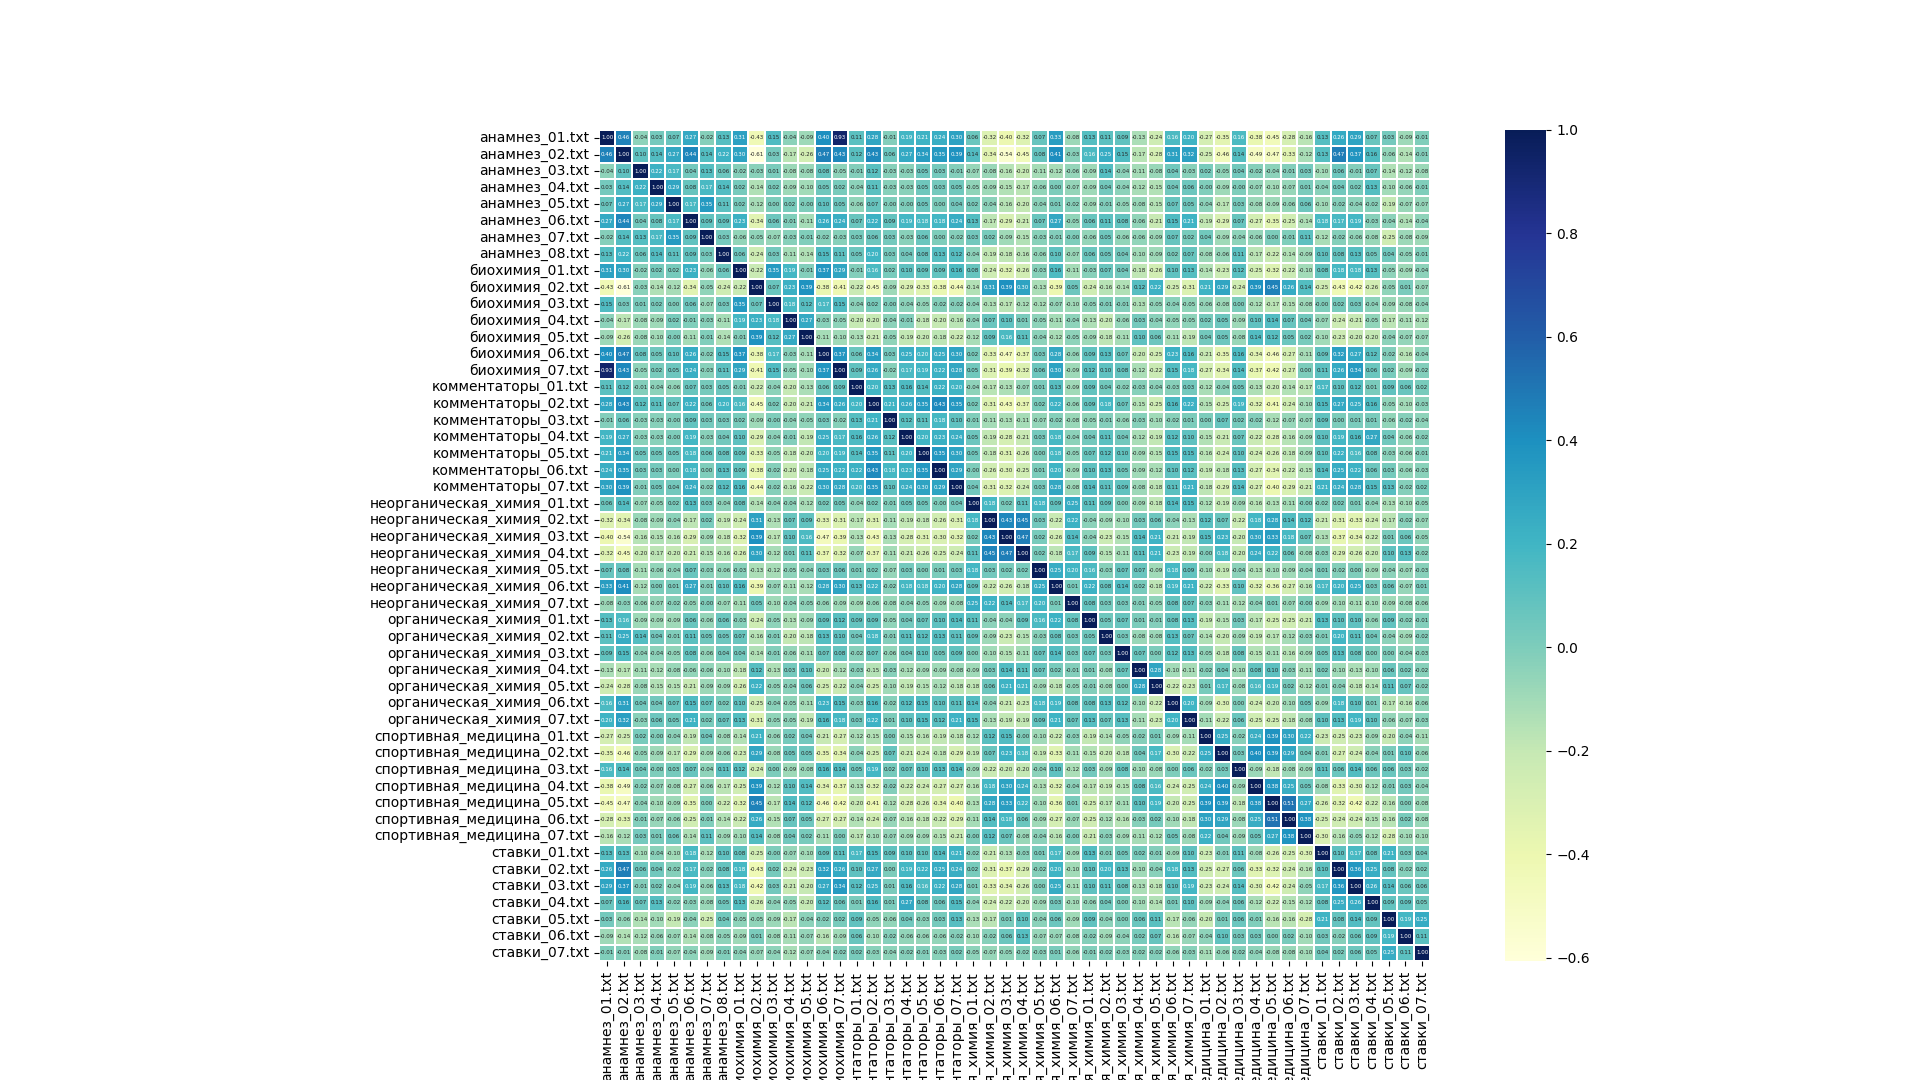
\includegraphics[width=1.1\linewidth]{C:/MGTU/baseAI/lr8_git/bag23u045/report/images/HeatmapCos.png}}
        а) До сокращения вектора 
    \end{minipage}
    \begin{minipage}[H]{0.5\linewidth}
        \center{\includegraphics[width=1.1\linewidth]{C:/MGTU/baseAI/lr10/bag23u045/report/results/Heatmap_dispersion_cosine.png}}
        б) После сокращения вектора 
    \end{minipage}
    \caption{Сравнение косинусным методом уменьшенного вектора с помощью диспресии}
    \label{fig:heatmapVarCos}
\end{figure}

\begin{figure}[H]
    \begin{minipage}[H]{0.5\linewidth}
        \center{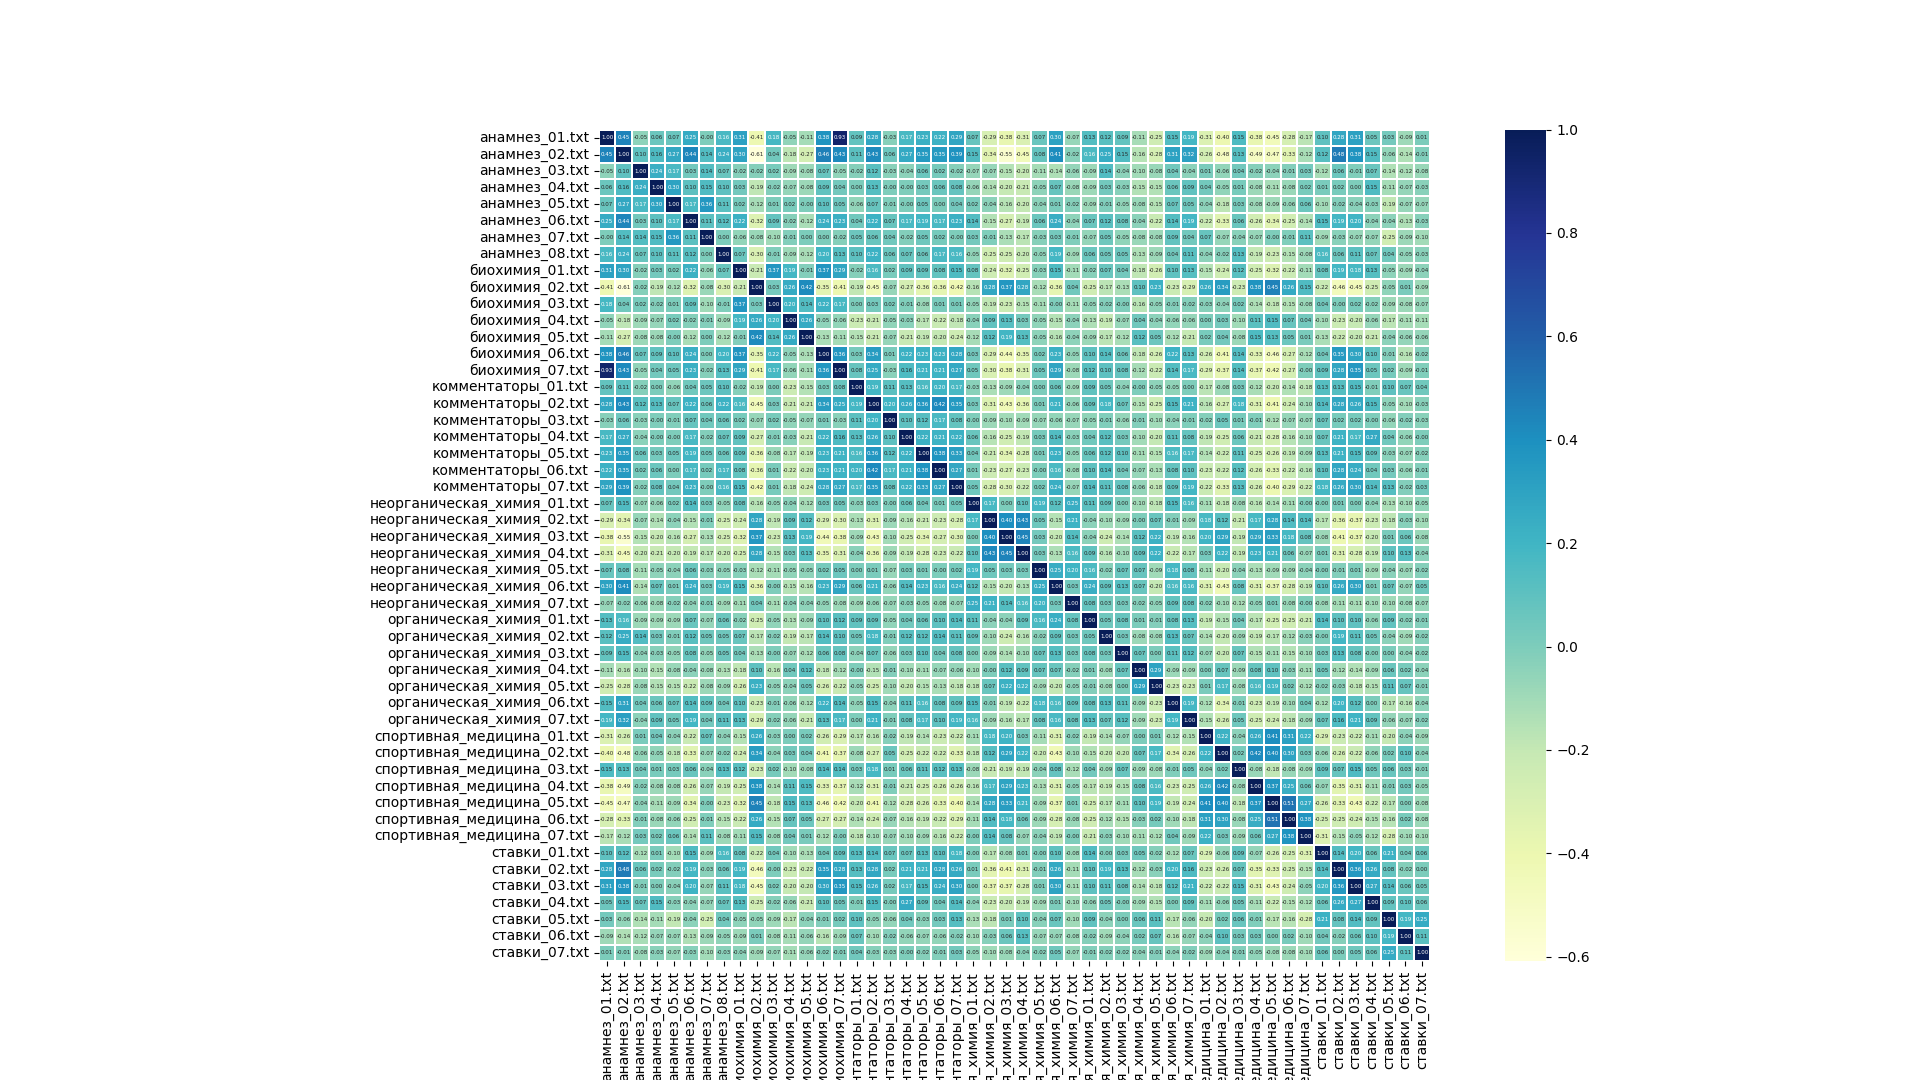
\includegraphics[width=1.1\linewidth]{C:/MGTU/baseAI/lr8_git/bag23u045/report/images/HeatmapPearson.png}}
        а) До сокращения вектора 
    \end{minipage}
    \begin{minipage}[H]{0.5\linewidth}
        \center{\includegraphics[width=1.1\linewidth]{C:/MGTU/baseAI/lr10/bag23u045/report/results/Heatmap_dispersion_pearson.png}}
        б) После сокращения вектора 
    \end{minipage}
    \caption{Сравнение методом Пирсона уменьшенного вектора с помощью диспресии}
    \label{fig:heatmapVarPear}
\end{figure}

\begin{figure}[H]
    \begin{minipage}[H]{0.5\linewidth}
        \center{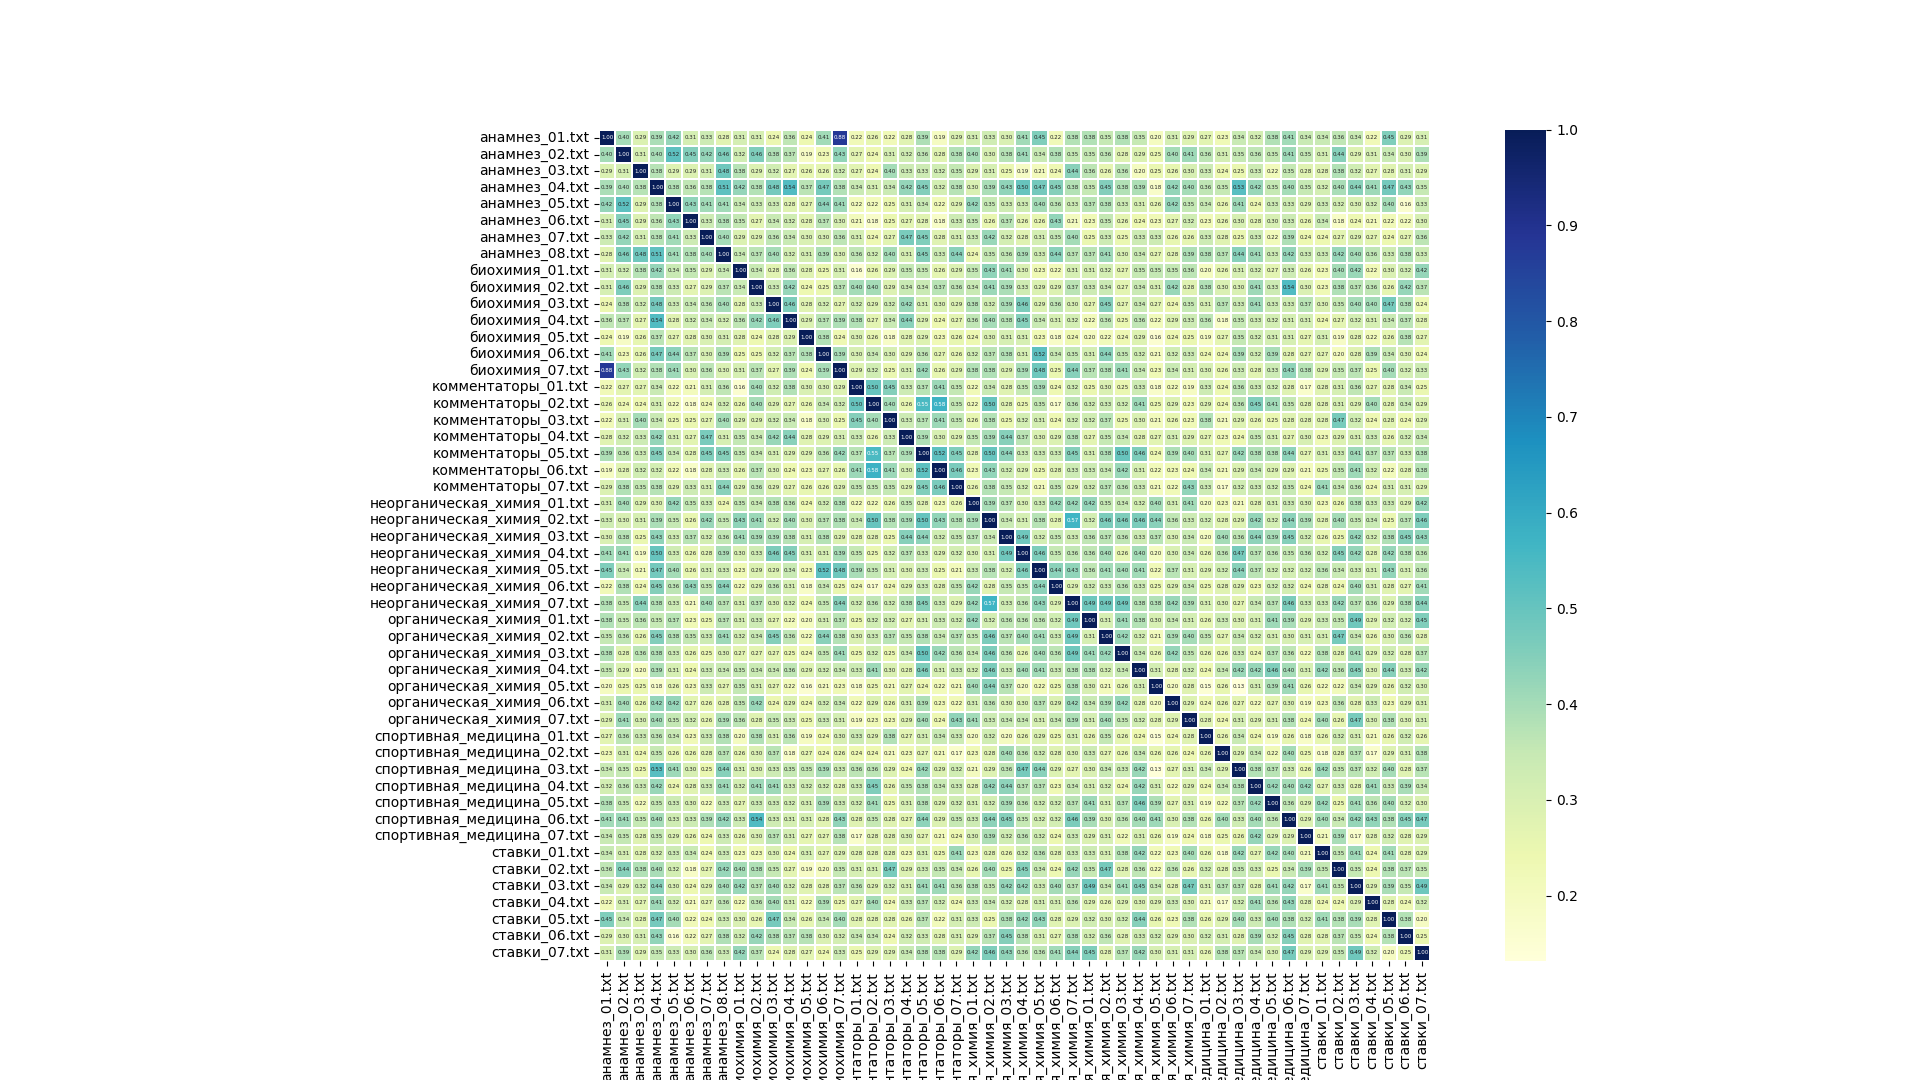
\includegraphics[width=1.1\linewidth]{C:/MGTU/baseAI/lr8_git/bag23u045/report/images/HeatmapJac.png}}
        а) До сокращения вектора 
    \end{minipage}
    \begin{minipage}[H]{0.5\linewidth}
        \center{\includegraphics[width=1.1\linewidth]{C:/MGTU/baseAI/lr10/bag23u045/report/results/Heatmap_covariance_jac.png}}
        б) После сокращения вектора 
    \end{minipage}
    \caption{Сравнение методом Жаккарда уменьшенного вектора с помощью ковариации}
    \label{fig:heatmapCovJac}
\end{figure}

\begin{figure}[H]
    \begin{minipage}[H]{0.5\linewidth}
        \center{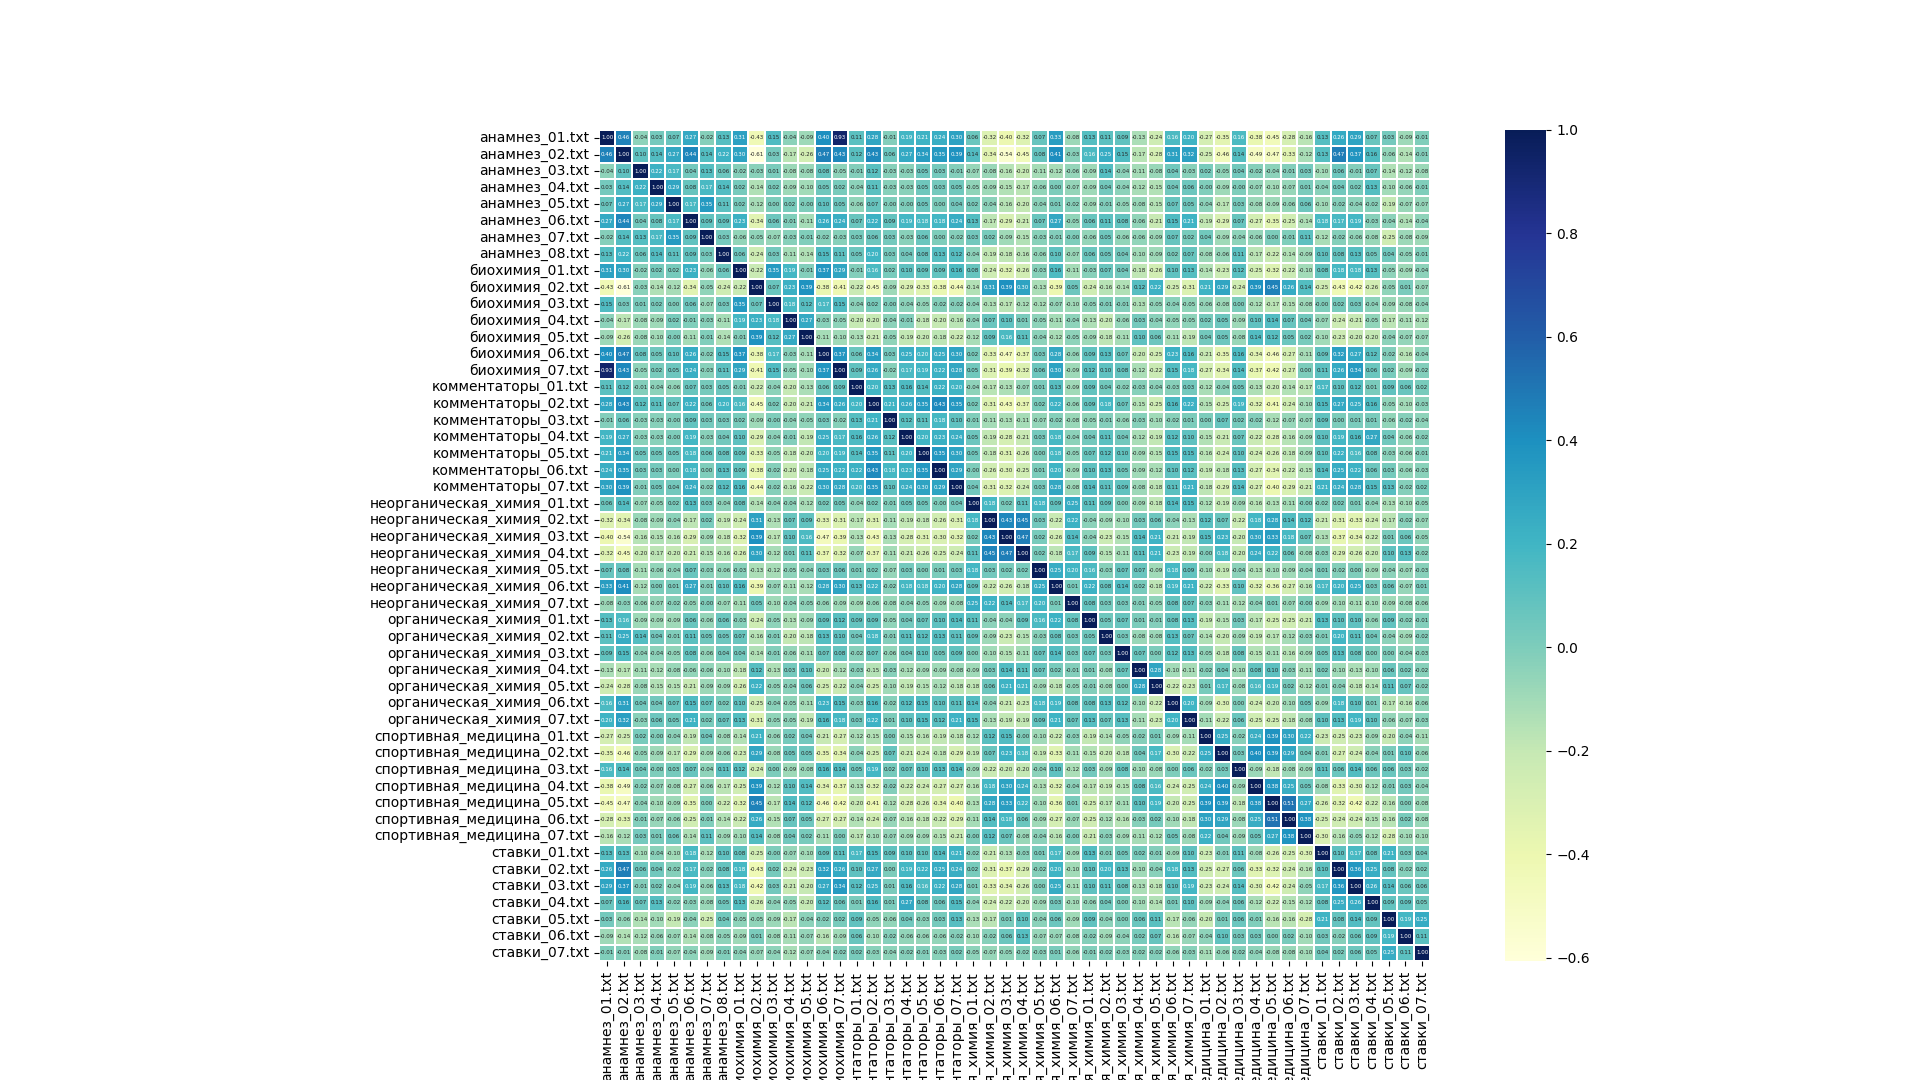
\includegraphics[width=1.1\linewidth]{C:/MGTU/baseAI/lr8_git/bag23u045/report/images/HeatmapCos.png}}
        а) До сокращения вектора 
    \end{minipage}
    \begin{minipage}[H]{0.5\linewidth}
        \center{\includegraphics[width=1.1\linewidth]{C:/MGTU/baseAI/lr10/bag23u045/report/results/Heatmap_covariance_cosine.png}}
        б) После сокращения вектора 
    \end{minipage}
    \caption{Сравнение косинусным методом уменьшенного вектора с помощью ковариации}
    \label{fig:heatmapCovCos}
\end{figure}

\begin{figure}[H]
    \begin{minipage}[H]{0.5\linewidth}
        \center{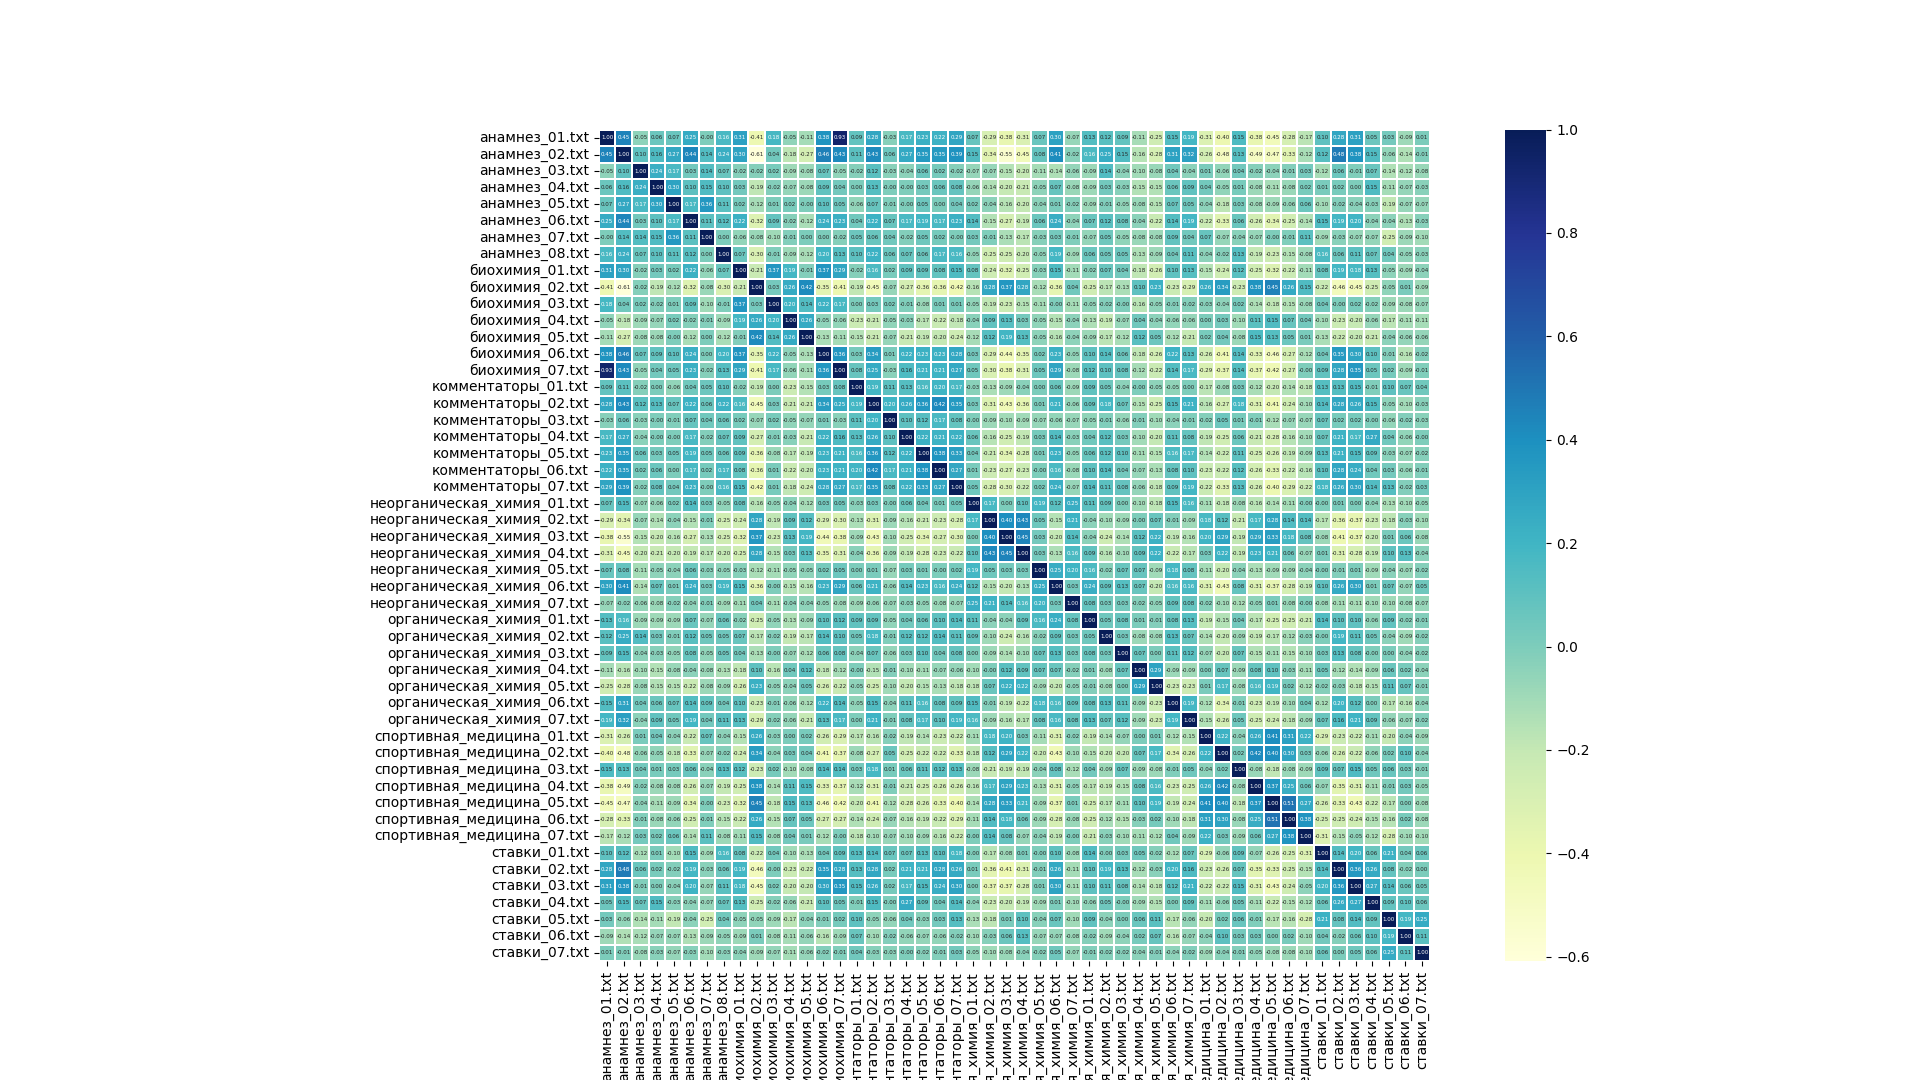
\includegraphics[width=1.1\linewidth]{C:/MGTU/baseAI/lr8_git/bag23u045/report/images/HeatmapPearson.png}}
        а) До сокращения вектора 
    \end{minipage}
    \begin{minipage}[H]{0.5\linewidth}
        \center{\includegraphics[width=1.1\linewidth]{C:/MGTU/baseAI/lr10/bag23u045/report/results/Heatmap_covariance_pearson.png}}
        б) После сокращения вектора 
    \end{minipage}
    \caption{Сравнение методом Пирсона уменьшенного вектора с помощью ковариации}
    \label{fig:heatmapCovPear}
\end{figure}

\begin{figure}[H]
    \begin{minipage}[H]{0.5\linewidth}
        \center{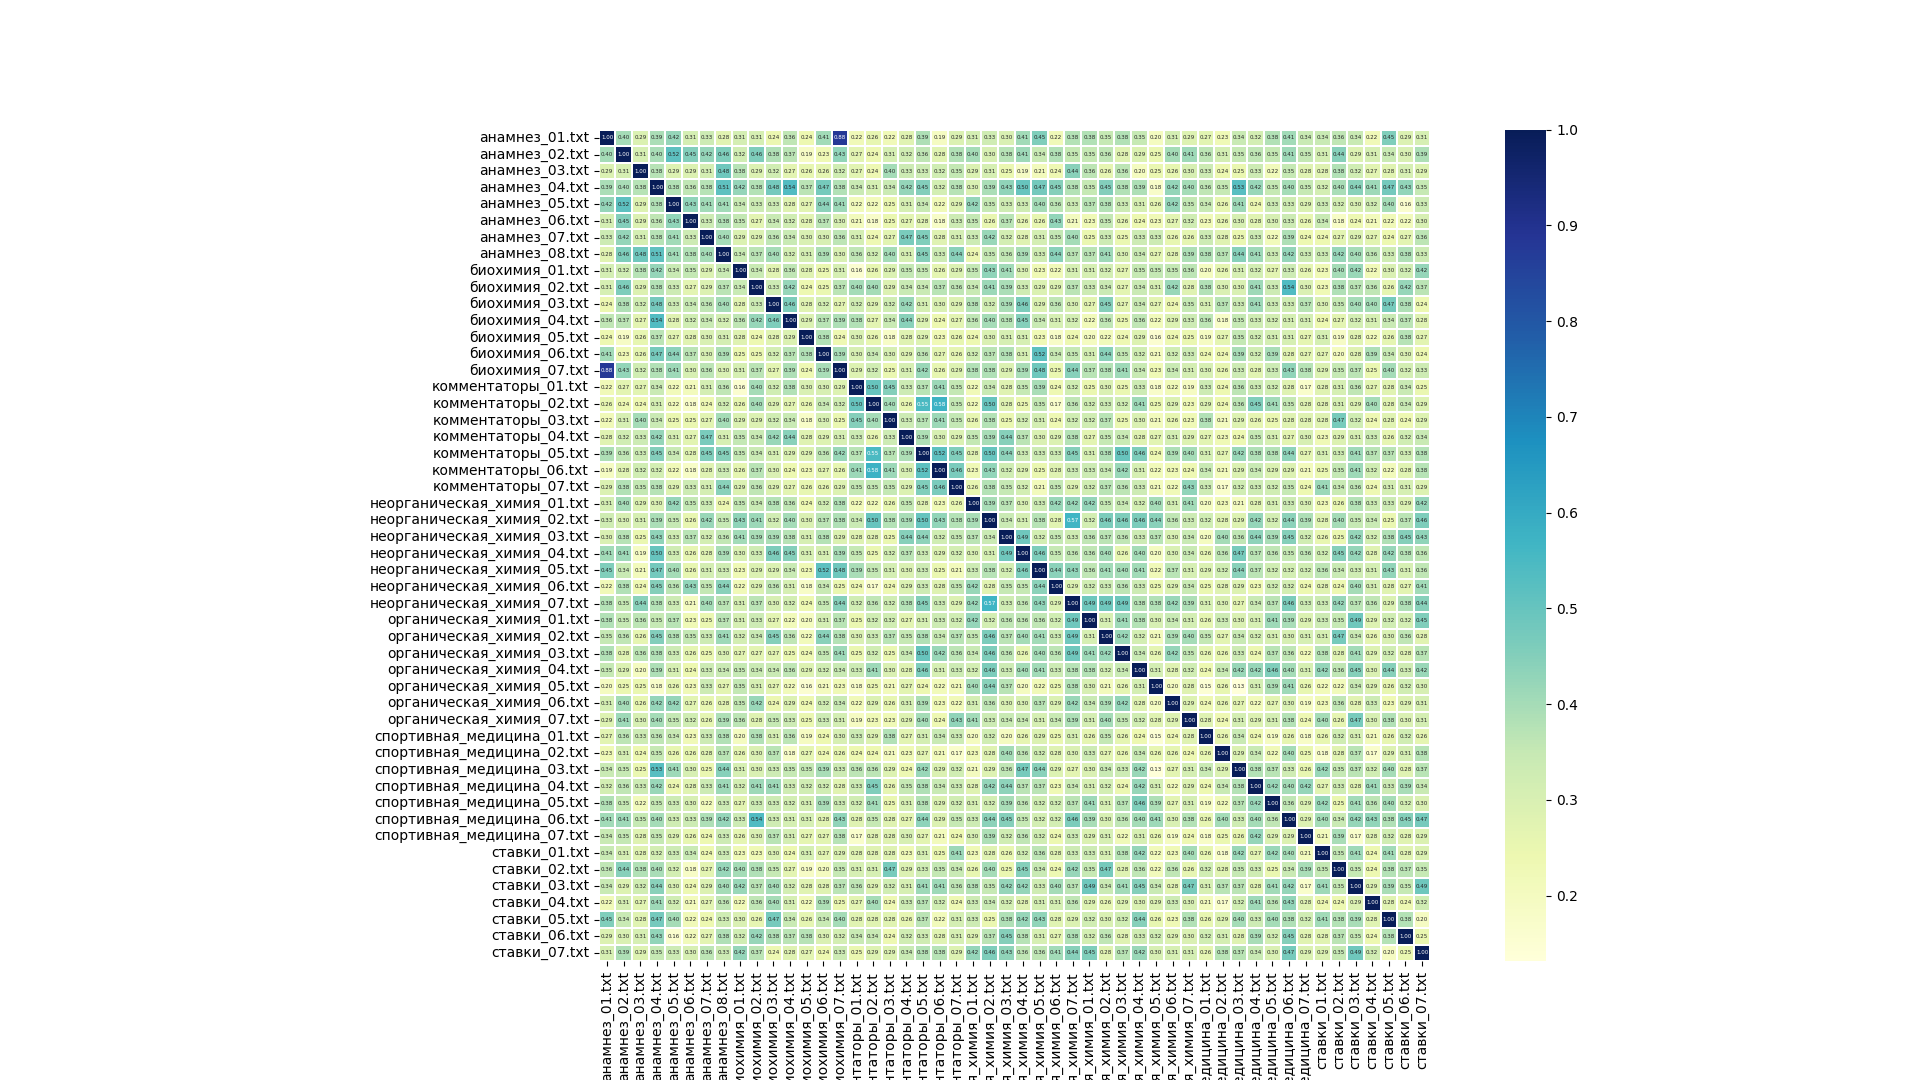
\includegraphics[width=1.1\linewidth]{C:/MGTU/baseAI/lr8_git/bag23u045/report/images/HeatmapJac.png}}
        а) До сокращения вектора 
    \end{minipage}
    \begin{minipage}[H]{0.5\linewidth}
        \center{\includegraphics[width=1.1\linewidth]{C:/MGTU/baseAI/lr10/bag23u045/report/results/Heatmap_pearson_jac.png}}
        б) После сокращения вектора 
    \end{minipage}
    \caption{Сравнение методом Жаккарда уменьшенного вектора с помощью корреляции Пирсона}
    \label{fig:heatmapPearJac}
\end{figure}

\begin{figure}[H]
    \begin{minipage}[H]{0.5\linewidth}
        \center{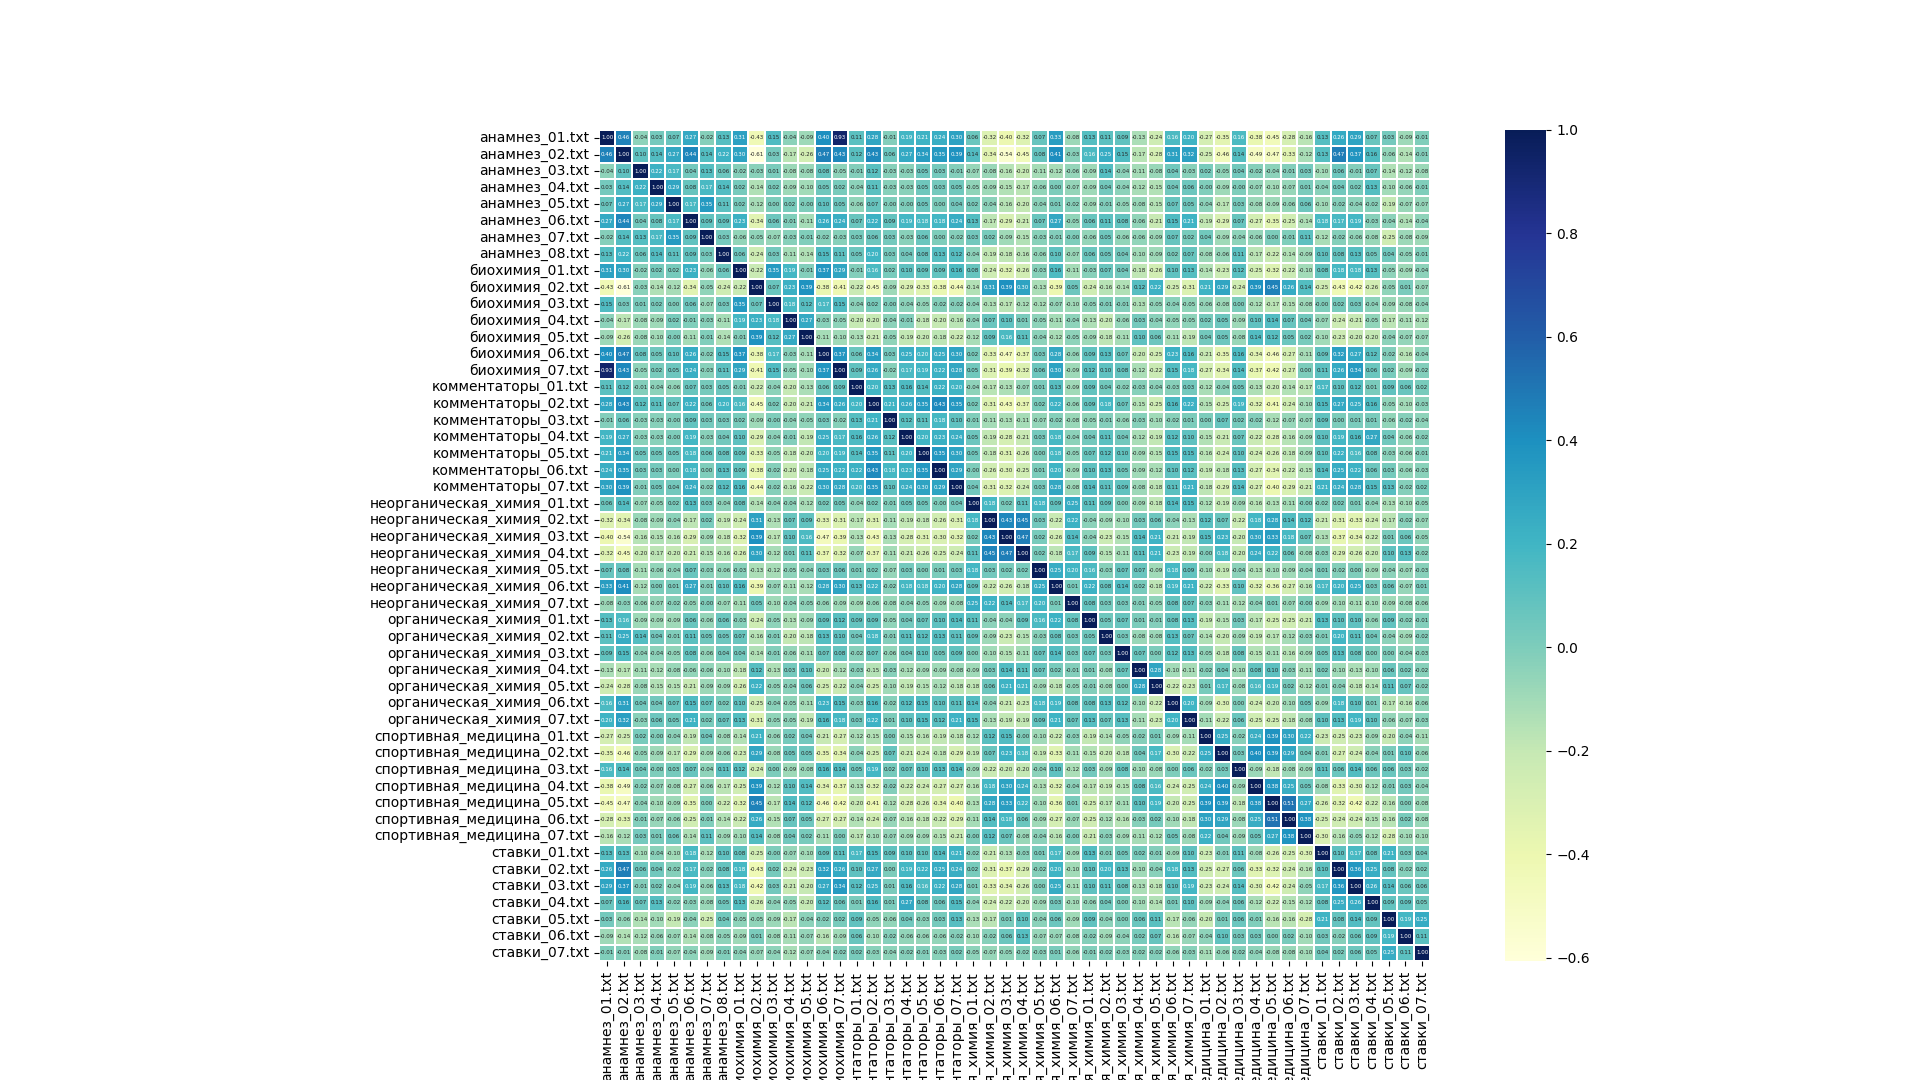
\includegraphics[width=1.1\linewidth]{C:/MGTU/baseAI/lr8_git/bag23u045/report/images/HeatmapCos.png}}
        а) До сокращения вектора 
    \end{minipage}
    \begin{minipage}[H]{0.5\linewidth}
        \center{\includegraphics[width=1.1\linewidth]{C:/MGTU/baseAI/lr10/bag23u045/report/results/Heatmap_pearson_cosine.png}}
        б) После сокращения вектора 
    \end{minipage}
    \caption{Сравнение косинусным методом уменьшенного вектора с помощью корреляции Пирсона}
    \label{fig:heatmapPearCos}
\end{figure}

\begin{figure}[H]
    \begin{minipage}[H]{0.5\linewidth}
        \center{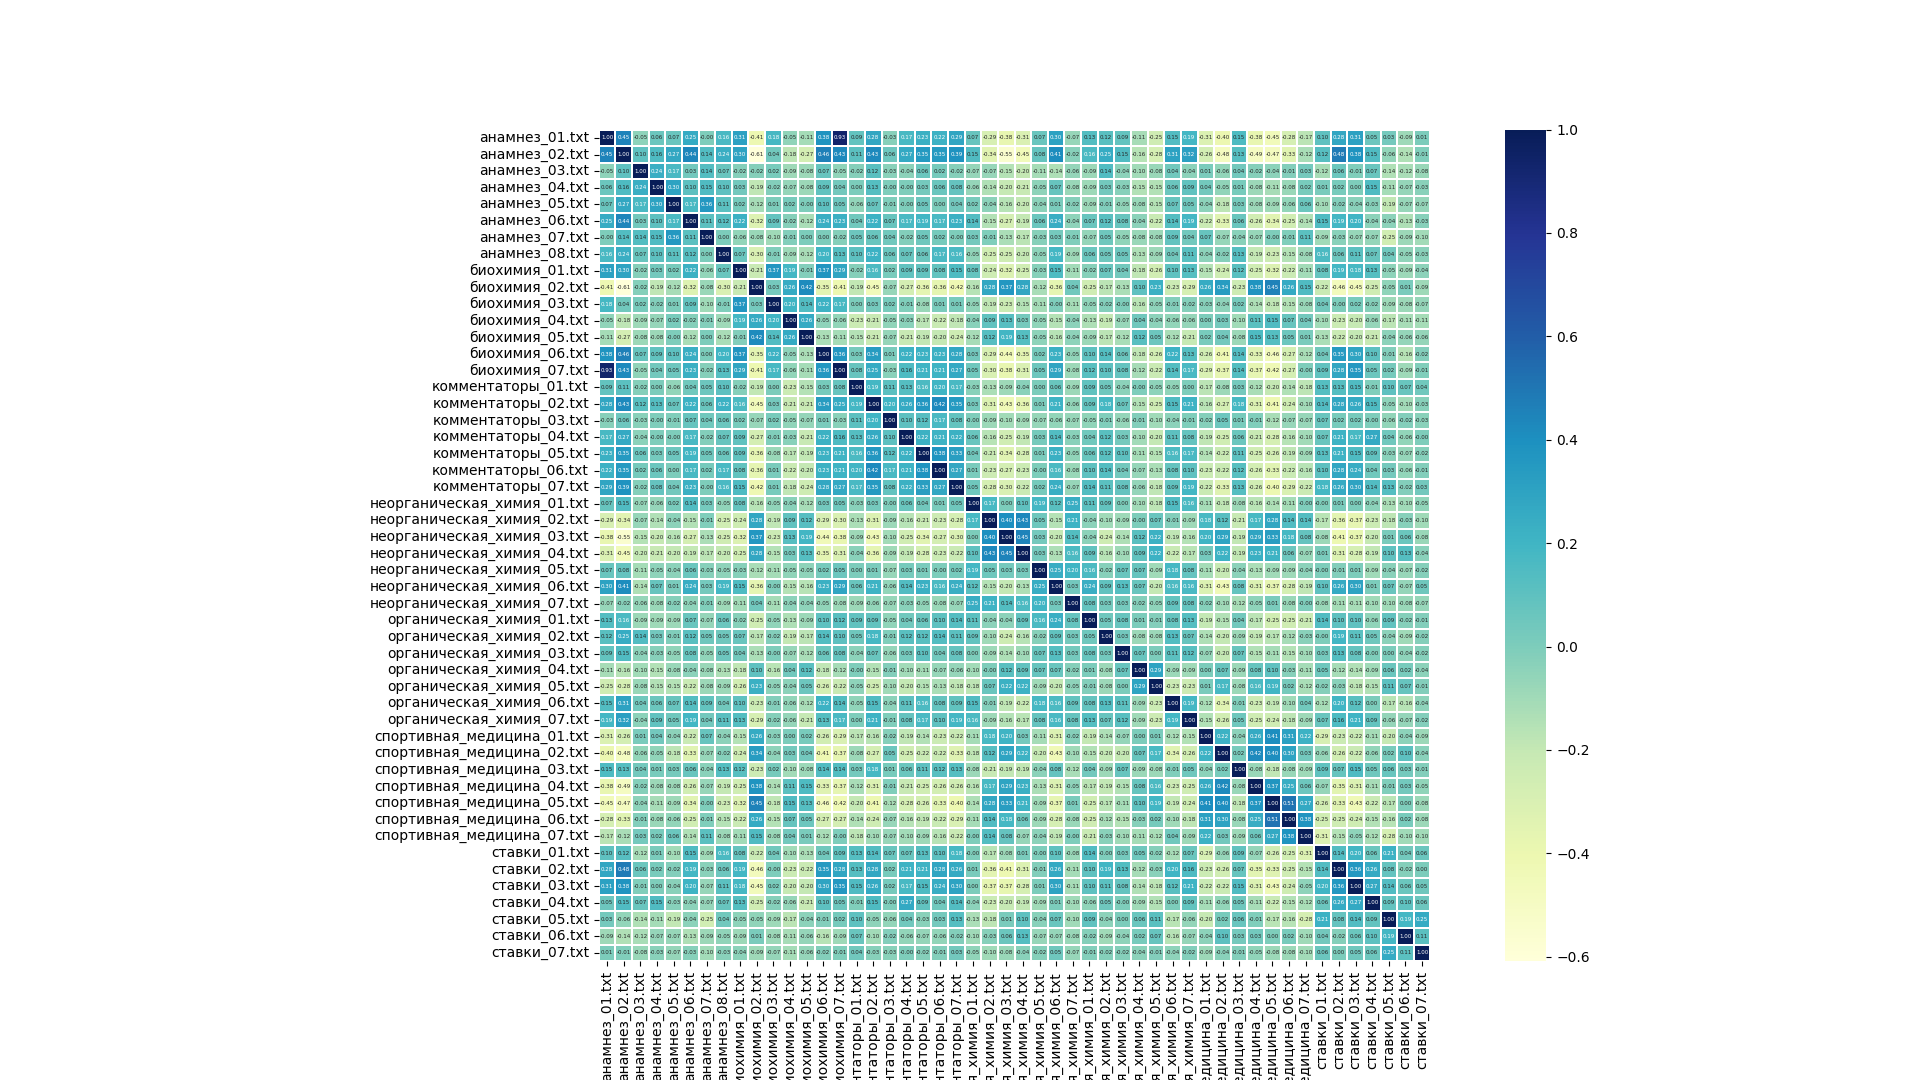
\includegraphics[width=1.1\linewidth]{C:/MGTU/baseAI/lr8_git/bag23u045/report/images/HeatmapPearson.png}}
        а) До сокращения вектора 
    \end{minipage}
    \begin{minipage}[H]{0.5\linewidth}
        \center{\includegraphics[width=1.1\linewidth]{C:/MGTU/baseAI/lr10/bag23u045/report/results/Heatmap_pearson_pearson.png}}
        б) После сокращения вектора 
    \end{minipage}
    \caption{Сравнение методом Пиросона уменьшенного вектора с помощью корреляции Пирсона}
    \label{fig:heatmapPearPear}
\end{figure}

\begin{figure}[H]
    \begin{minipage}[H]{0.5\linewidth}
        \center{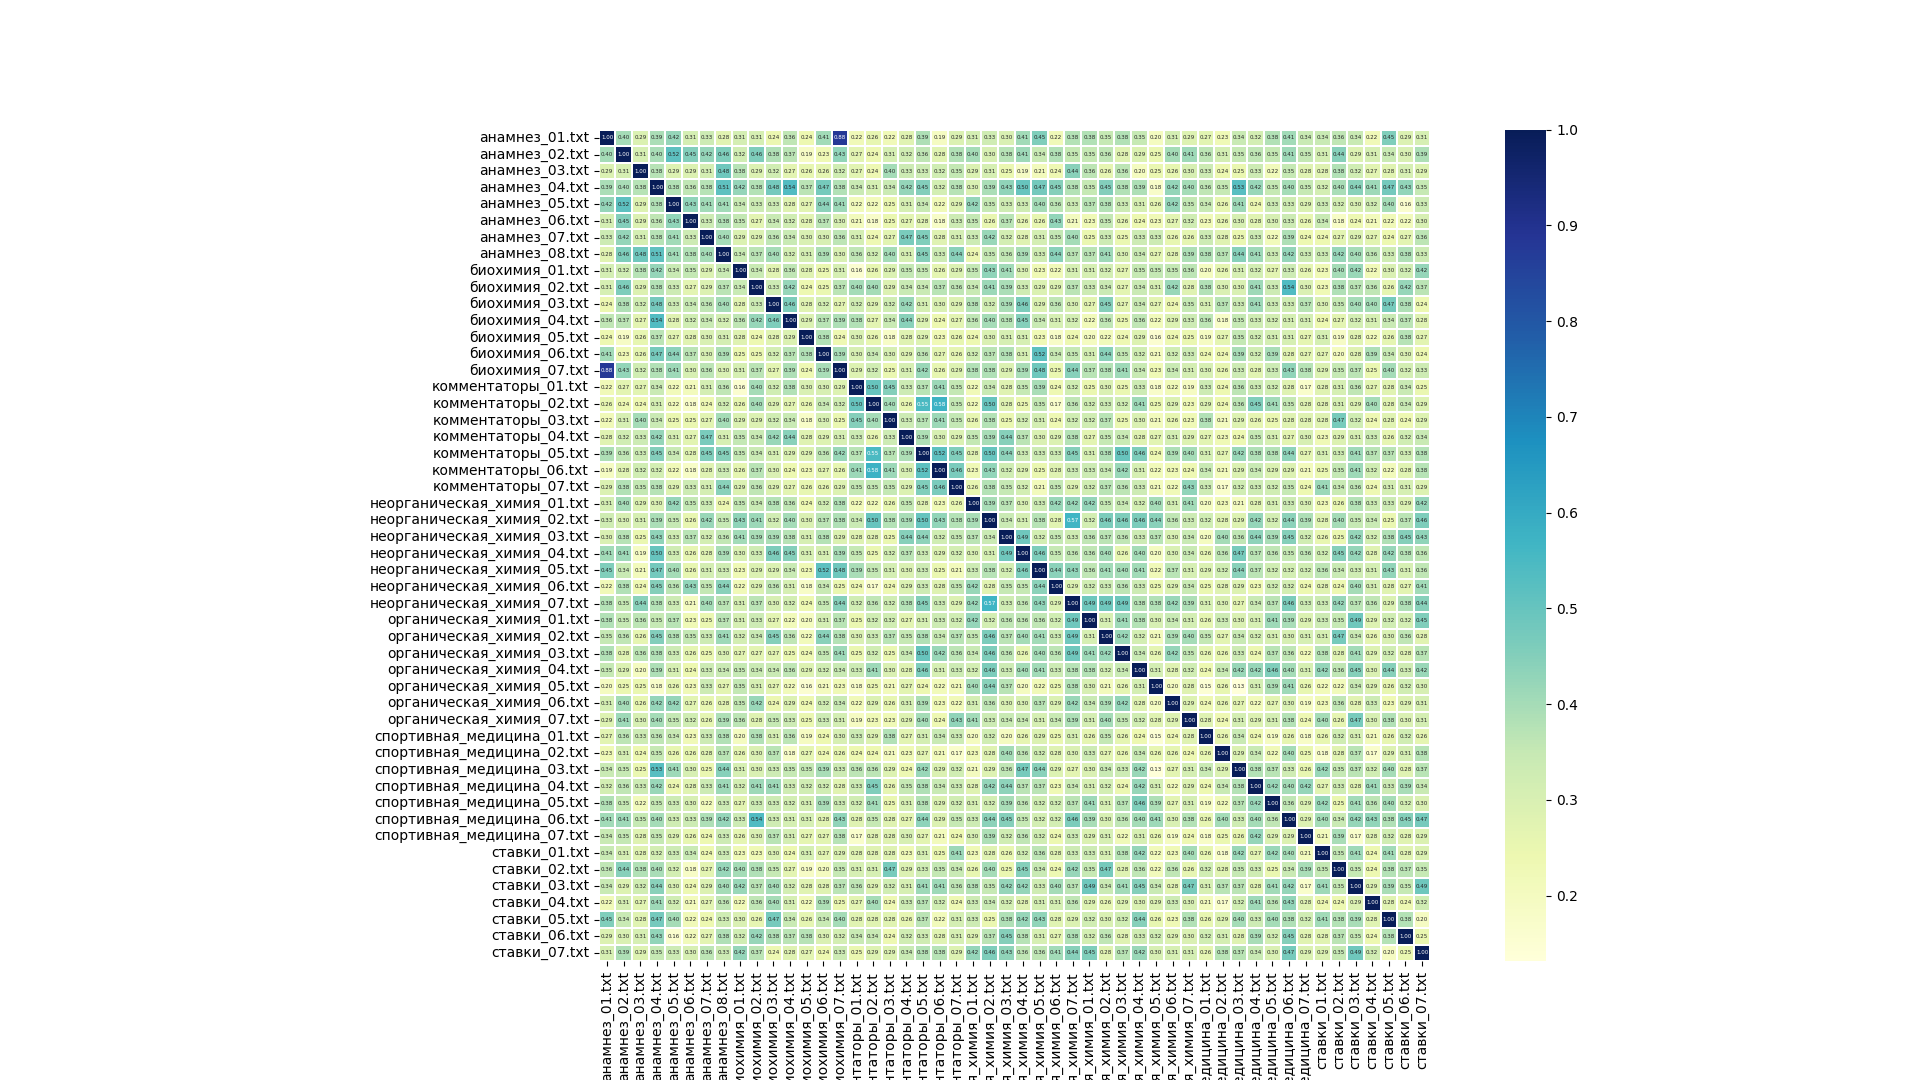
\includegraphics[width=1.1\linewidth]{C:/MGTU/baseAI/lr8_git/bag23u045/report/images/HeatmapJac.png}}
        а) До сокращения вектора 
    \end{minipage}
    \begin{minipage}[H]{0.5\linewidth}
        \center{\includegraphics[width=1.1\linewidth]{C:/MGTU/baseAI/lr10/bag23u045/report/results/Heatmap_spearman_jac.png}}
        б) После сокращения вектора 
    \end{minipage}
    \caption{Сравнение методом Жаккарда уменьшенного вектора с помощью корреляции Спирмена}
    \label{fig:heatmapSpearJac}
\end{figure}

\begin{figure}[H]
    \begin{minipage}[H]{0.5\linewidth}
        \center{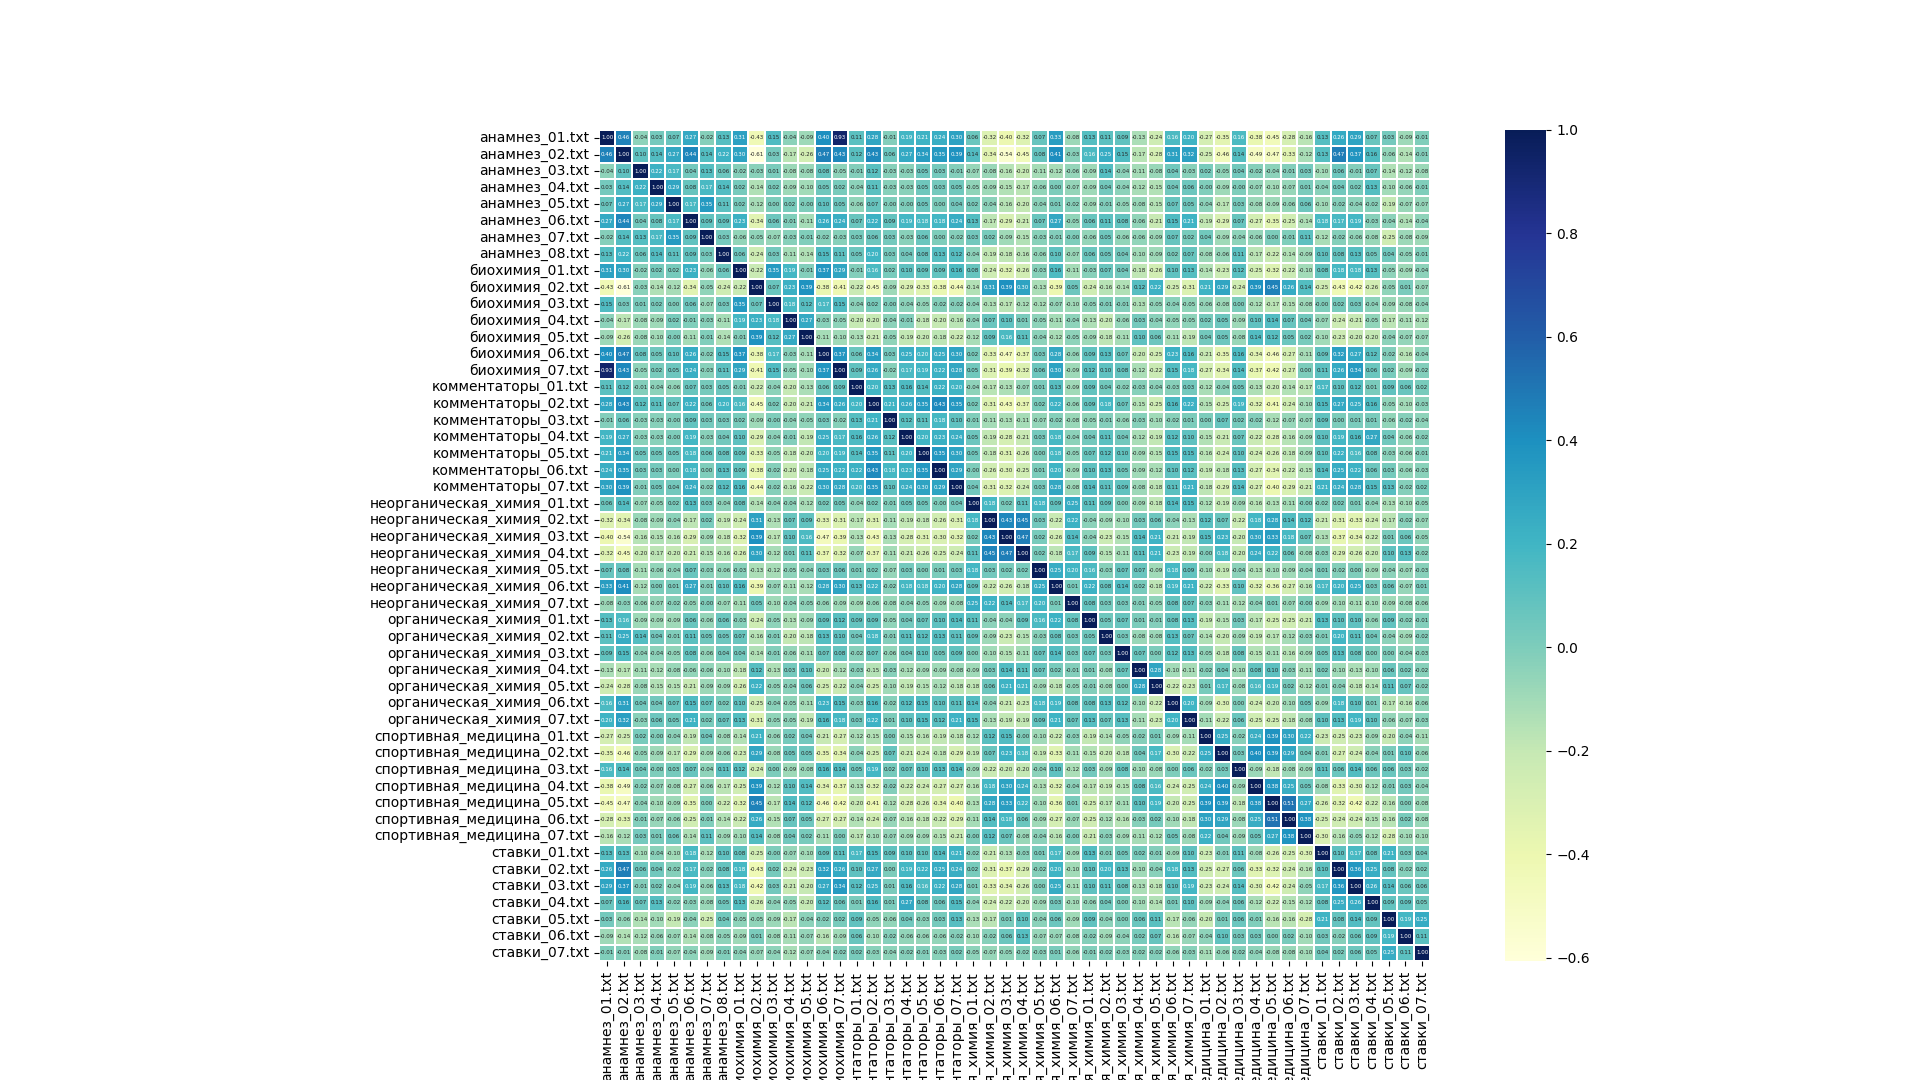
\includegraphics[width=1.1\linewidth]{C:/MGTU/baseAI/lr8_git/bag23u045/report/images/HeatmapCos.png}}
        а) До сокращения вектора 
    \end{minipage}
    \begin{minipage}[H]{0.5\linewidth}
        \center{\includegraphics[width=1.1\linewidth]{C:/MGTU/baseAI/lr10/bag23u045/report/results/Heatmap_spearman_cosine.png}}
        б) После сокращения вектора 
    \end{minipage}
    \caption{Сравнение косинусным методом уменьшенного вектора с помощью корреляции Спирмена}
    \label{fig:heatmapSpearCos}
\end{figure}

\begin{figure}[H]
    \begin{minipage}[H]{0.5\linewidth}
        \center{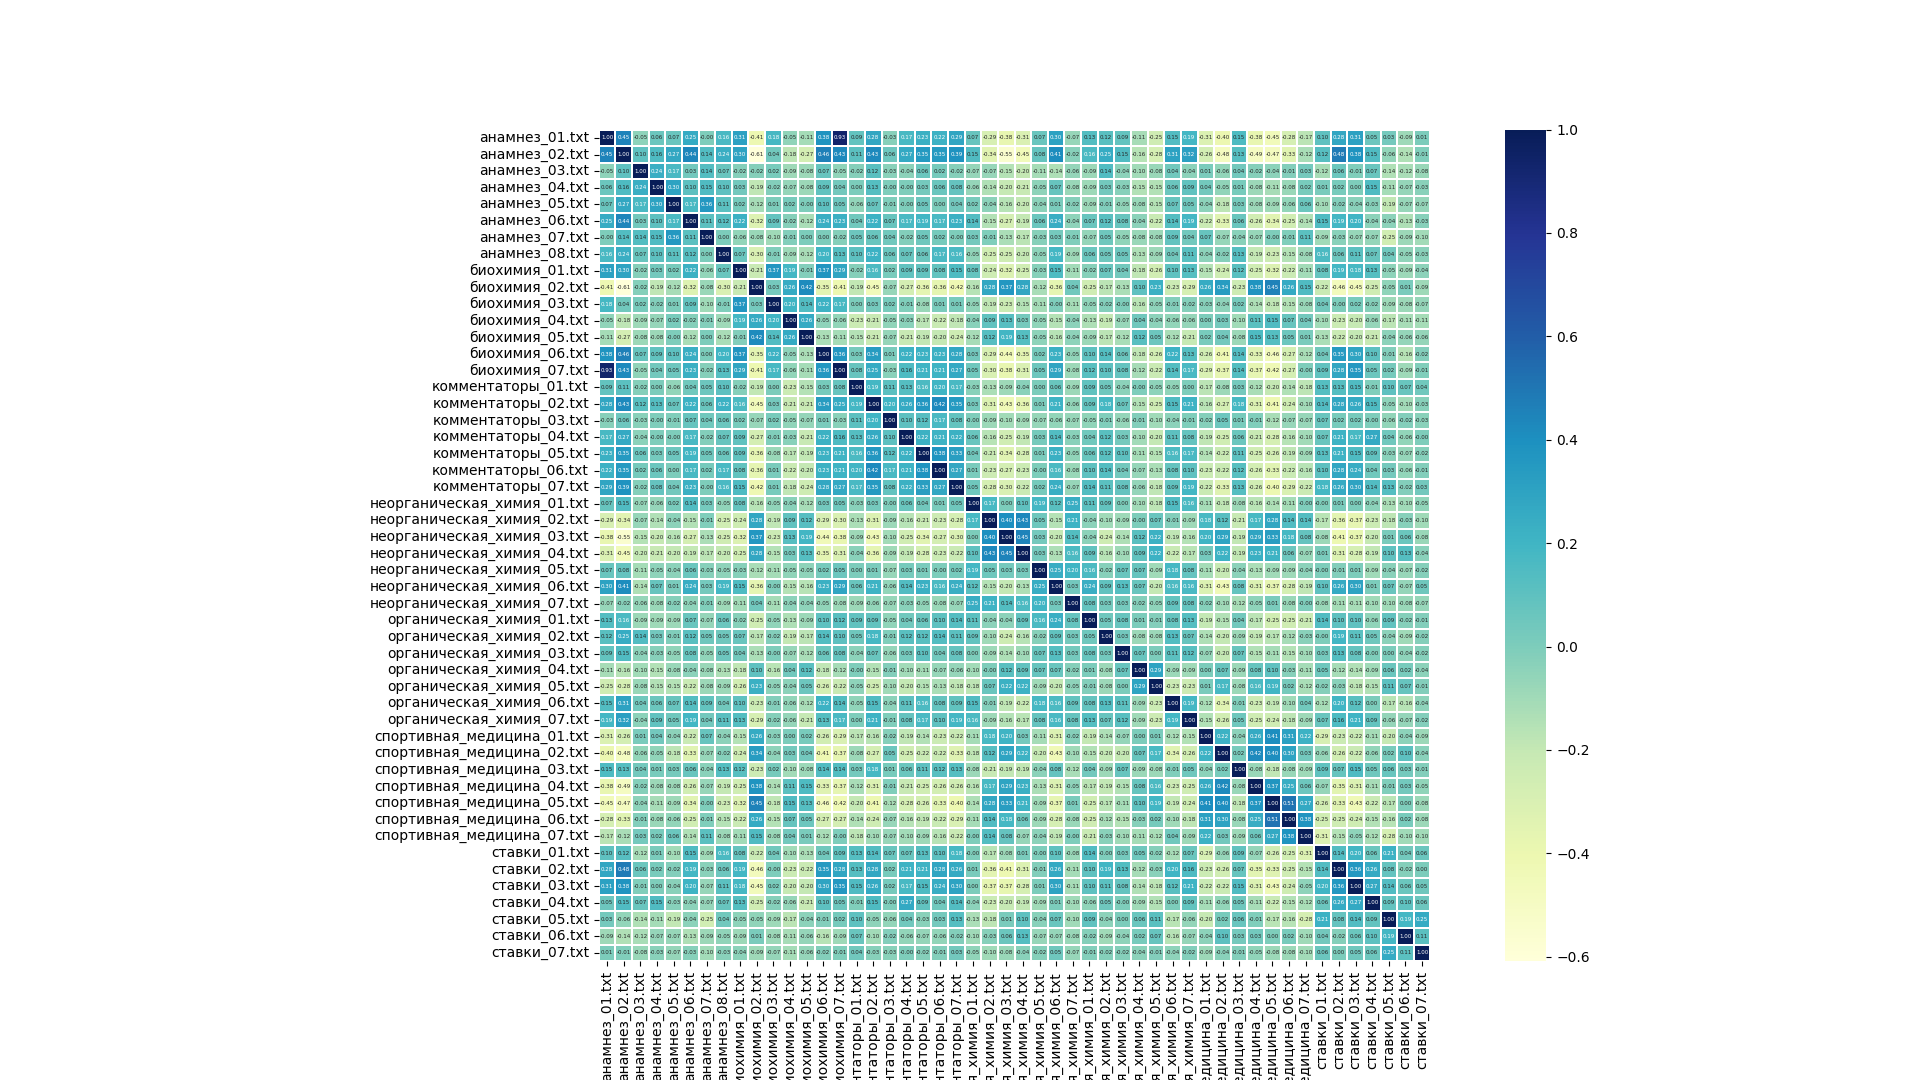
\includegraphics[width=1.1\linewidth]{C:/MGTU/baseAI/lr8_git/bag23u045/report/images/HeatmapPearson.png}}
        а) До сокращения вектора 
    \end{minipage}
    \begin{minipage}[H]{0.5\linewidth}
        \center{\includegraphics[width=1.1\linewidth]{C:/MGTU/baseAI/lr10/bag23u045/report/results/Heatmap_spearman_pearson.png}}
        б) После сокращения вектора 
    \end{minipage}
    \caption{Сравнение методом Пирсона уменьшенного вектора с помощью корреляции Спирмена}
    \label{fig:heatmapSpearPear}
\end{figure}

\section{Вывод}

Метрика Жаккарда оказалась менее подходящей для анализа: тепловая карта получилась слишком бледной, 
что затрудняет визуальную оценку результатов. В то же время косинусная метрика и корреляция Пирсона дали почти одинаковые результаты, 
что позволяет считать их взаимозаменяемыми для этого исследования.

\clearpage
